\documentclass[12pt]{article}
\usepackage{times}
\usepackage[english]{babel}
\usepackage[utf8x]{inputenc}
\usepackage[colorinlistoftodos]{todonotes}
\usepackage[margin=1in]{geometry}
\usepackage{graphicx}
\usepackage{epstopdf}
\usepackage{cite}
\usepackage{listings}
\usepackage{dtklogos}
\usepackage{wrapfig}
\usepackage{subfigure}
\usepackage{amsmath}
\usepackage{amsthm}
\usepackage{amssymb}
\usepackage{amscd}
\usepackage{caption}
\usepackage{etoolbox}
\usepackage{fancyhdr}
\usepackage{stackengine}
\usepackage[export]{adjustbox}
\patchcmd{\thebibliography}{\section*{\refname}}{}{}{}
\usepackage[document]{ragged2e}    %This causes text to left align
\usepackage[colorlinks=true, linkcolor=black,citecolor=black,urlcolor=blue]{hyperref}
\bibliographystyle{IEEEtran}
\extrafloats{100}
\DeclareGraphicsRule{.tif}{png}{.png}{`convert #1 `dirname #1`/`basename #1 .tif`.png}

\title{MCHE 357: Lab 2}

\begin{document}
\lefthyphenmin3
\righthyphenmin4
% \pretolerance=2000
% \tolerance=500 
% \emergencystretch=10pt
%\raggedright     %Stops LaTeX from automatically hyphenating the right margin to fit better
%Combine this with \usepackage[document]{ragged2e} to get a text align left similar to natural MS Word


%-------------------------------------------------------------
%Start of Paper
%-------------------------------------------------------------

%%%%%%%%%%%%%%%%%%%%%%%%%%%%%%%%%%%%%%%%%%%%%%%%%%%%%%
%%%%%%%%%%%%%%%%%%%%%%% TITLE PAGE %%%%%%%%%%%%%%%%%%%%%%%%
%%%%%%%%%%%%%%%%%%%%%%%%%%%%%%%%%%%%%%%%%%%%%%%%%%%%%%

\begin{titlepage}

\newcommand{\HRule}{\rule{\linewidth}{0.5mm}} % Defines a new command for the horizontal lines, change thickness here

\center % Center everything on the page
 
%----------------------------------------------------------------------------------------
%	Heading Section
%----------------------------------------------------------------------------------------

\textsc{\LARGE University of Louisiana at Lafayette}\\[1.5cm] % Name of your university/college
\textsc{\Large Measurements and Instrumentation}\\[0.5cm] % Major heading such as course name
\textsc{\large MCHE 357}\\[0.5cm] % Minor heading such as course title

%----------------------------------------------------------------------------------------
%	Title Section
%----------------------------------------------------------------------------------------

\HRule \\[0.4cm]
{ \huge \bfseries Lab 2}\\[0.4cm] % Title of your document
\HRule \\[1.5cm]
 
%----------------------------------------------------------------------------------------
%	Author Section
%----------------------------------------------------------------------------------------

\begin{minipage}{0.4\textwidth}
\begin{flushleft} \large
\emph{Author:}\\
\textsc{Matthew J. Begneaud} \\% Your name
\end{flushleft}
\end{minipage}
~
\begin{minipage}{0.4\textwidth}
\begin{flushright} \large
\emph{Professor:} \\
\textsc{Dr. Mostafa A. Elsayed} % Supervisor's Name
\end{flushright}
\end{minipage}\\[1.5cm]

% If you don't want a supervisor, uncomment the two lines below and remove the section above
%\Large \emph{Author:}\\
%John \textsc{Smith}\\[3cm] % Your name

%----------------------------------------------------------------------------------------
%	Date Section
%----------------------------------------------------------------------------------------

{\textsc{\large \today}}\\[0.5cm] % Date, change the \today to a set date if you want to be precise


%----------------------------------------------------------------------------------------
%	Group Section
%----------------------------------------------------------------------------------------

\textsc{\large Group:}\\[0.1cm]
\textsc{Ronald Kisor}\\
\textsc{Chandler Lagarde}\\
\textsc{Somto Umeokafor}
\\[0.5cm]

%----------------------------------------------------------------------------------------
%	Logo Section
%----------------------------------------------------------------------------------------


\includegraphics[width=5in]{UL_logo.jpg}\\[1cm] % Include a department/university logo - this will require the graphicx package
 
%----------------------------------------------------------------------------------------

\vfill % Fill the rest of the page with whitespace

\end{titlepage}

%%%%%%%%%%%%%%%%%%%%%%%%%%%%%%%%%%%%%%%%%%%%%%%%%%%%%%
%%%%%%%%%%%%%%%%%%%%%%% TABLE OF CONTENTS %%%%%%%%%%%%%%%%%%%
%%%%%%%%%%%%%%%%%%%%%%%%%%%%%%%%%%%%%%%%%%%%%%%%%%%%%%

\tableofcontents

\listoffigures

\bigskip


\section*{\fontsize{12}{12}\selectfont \large List of Symbols}
\addcontentsline{toc}{section}{List of Symbols} % Add for each section
$V$ = Voltage (Volts)\\
$L$ = Inductance (Henries)\\
$R$ = Resistance (Ohms)\\
$q$ = Charge (Coulombs)\\
$q'$ = First derivative of charge (current)\\
$q''$ = Second derivative of charge (change in current)\\
$w_{n}$ = Natural frequency (Radians/second)\\

\newpage

%%%%%%%%%%%%%%%%%%%%%%%%%%%%%%%%%%%%%%%%%%%%%%%%%%%%%%
%%%%%%%%%%%%%%%%%%%%%%% REPORT %%%%%%%%%%%%%%%%%%%%%%%%%%
%%%%%%%%%%%%%%%%%%%%%%%%%%%%%%%%%%%%%%%%%%%%%%%%%%%%%%


\section*{\fontsize{12}{12}\selectfont \large Introduction}
\addcontentsline{toc}{section}{Introduction} % Add for each section
This lab served as an introduction to the principles of RLC circuits. These circuits contain three main devices: resistance, capacitance, and inductance. These devices are placed in series to form a circuit who's behavior can be described with a differential equation. These types of circuits are the foundation of many devices, such as radio tuners. 



\section*{\fontsize{12}{12}\selectfont \large Theory}
\addcontentsline{toc}{section}{Theory} % Add for each section
The three main characteristics of electrical components must be understood to analyze RLC circuits. Resistance is a quality of a component which measures the blocking of current through the device. Capacitance is the ability of a device to store charge. Inductance is the characteristic of a device that reacts to changes in current. Each of these characteristics are analogous to mechanical properties. An inductance is analogous to inertia, or mass, resistance is analogous to dampening, and capacitance is analogous to a spring. Making a circuit with all three types of devices results in a system similar to a simple mechanical vibrating system with a mass, dampener, and spring. The equation of an RLC circuit is therefore similar to the basic vibration equation, and is shown in Equation 1.
\bigskip

If the input to an RLC circuit is sinusoidal, the output will also be sinusoidal, but will be either out of phase or in phase with the input. Whether the output is in phase or out of phase with the input depends mainly on the natural frequency of the circuit. If the input frequency is below the natural frequency of the circuit, the output will lag the input. If the input frequency is above the natural frequency, then the output will lead the input. However, if the frequency of the input matches the natural frequency of the circuit, the output will be in phase with the input. Commonly, the inductance of an RLC circuit is constant, and the resistance will be changed via a potentiometer in order to change the amplitude of the output. The capacitance can also typically be variable, which allows the user to change the natural frequency of the system, which is what happens when tuning a radio. These variances can be useful in many circuit applications.
\bigskip
 
 % Equations 1 and 2
 \begin{equation}
V = Lq'' + Rq' + \frac{1}{C}q
 \end{equation}
 \bigskip

\begin{equation}
w_{n} = \sqrt{\frac{1}{LC}}
\end{equation}

\newpage


\section*{\fontsize{12}{12}\selectfont \large Procedure \& Analysis}
\addcontentsline{toc}{section}{Procedure \& Analysis} % Add for each section
An RLC circuit was configured in Multisim, shown in Figure 1. The input was varied with a function generator, and the output was measured with an oscilloscope. The results from the oscilloscope were plotted at different frequencies and resistances, and are shown in Figures 2 through 8. In Figures 2 through 6, it is seen that when input frequency is held constant and the resistance changes, the amplitude changes. This result agrees with what was stated in the previous section. The input/output graphs at different frequencies were also plotted, shown in Figures 9 through 11.
\bigskip

% Multisim figures
\begin{figure}[h!] %  figure placement: here, top, bottom, or page
   \centering
   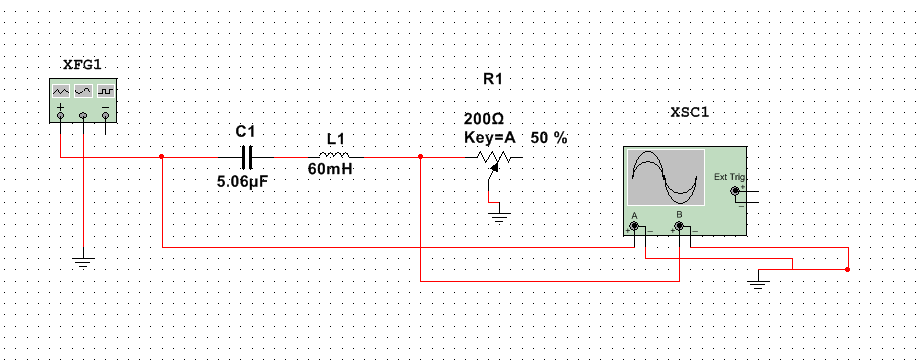
\includegraphics[width=5.5in]{Oscilloscope_Circuit.PNG} 
   \caption{Multisim RLC Circuit}
   \label{fig:example}
\end{figure}
\bigskip


\begin{figure}[h!] %  figure placement: here, top, bottom, or page
   \centering
   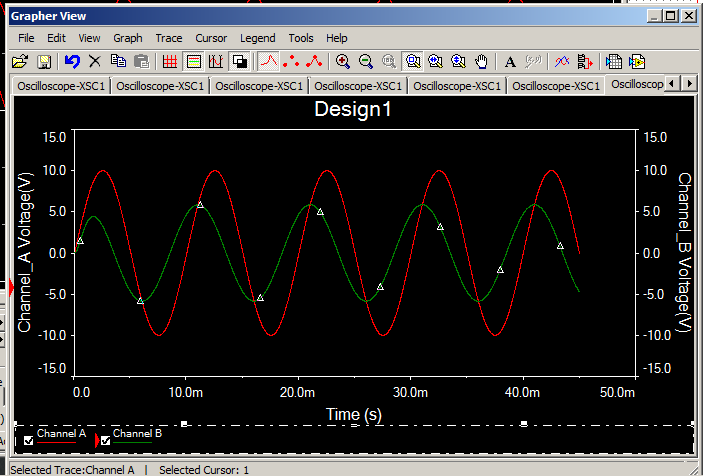
\includegraphics[width=5in]{100hz_0r.PNG} 
   \caption{RLC circuit at 100 Hertz and R = 0 Ohms}
   \label{fig:example}
\end{figure}

\newpage

\begin{figure}[h!] %  figure placement: here, top, bottom, or page
   \centering
   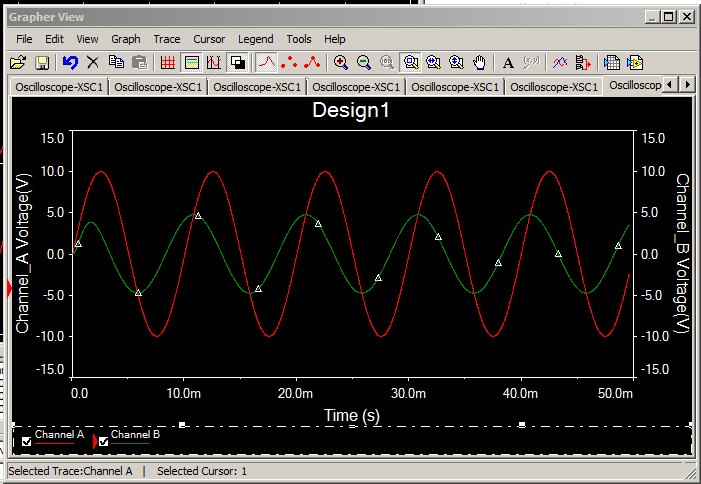
\includegraphics[width=5in]{100hz_25r.PNG} 
   \caption{RLC circuit at 100 Hertz and R = 25 Ohms}
   \label{fig:example}
\end{figure}
\bigskip

\begin{figure}[h!] %  figure placement: here, top, bottom, or page
   \centering
   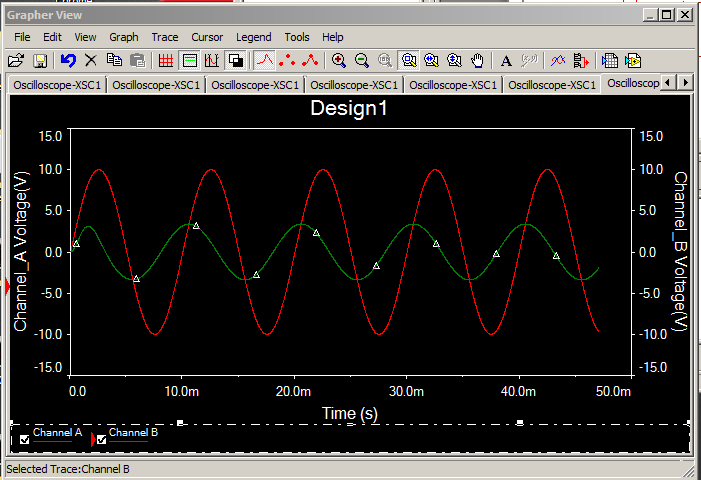
\includegraphics[width=5in]{100hz.PNG} 
   \caption{RLC circuit at 100 Hertz and R = 50 Ohms}
   \label{fig:example}
\end{figure}
\bigskip

\newpage

\begin{figure}[h!] %  figure placement: here, top, bottom, or page
   \centering
   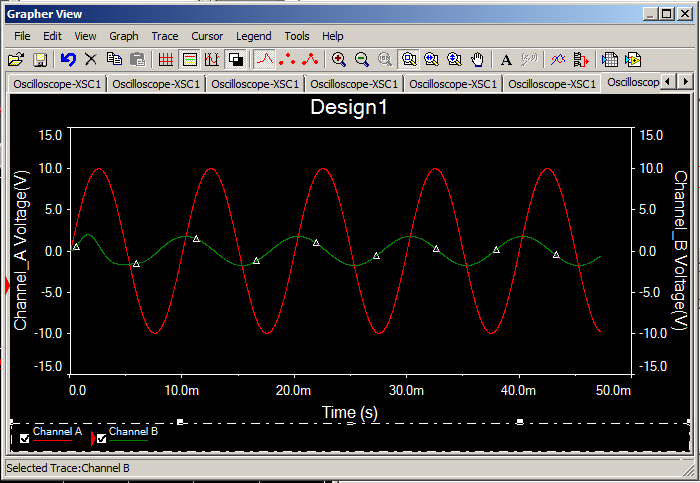
\includegraphics[width=5in]{100hz_75r.PNG} 
   \caption{RLC circuit at 100 Hertz and R = 75 Ohms}
   \label{fig:example}
\end{figure}
\bigskip

\begin{figure}[h!] %  figure placement: here, top, bottom, or page
   \centering
   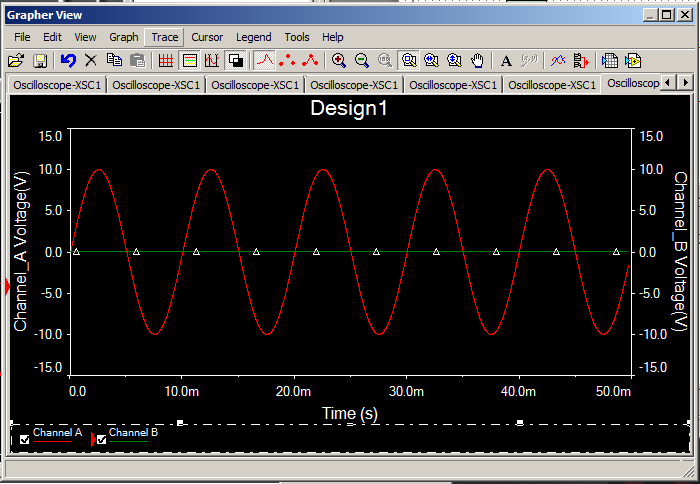
\includegraphics[width=5in]{100hz_100r.PNG} 
   \caption{RLC circuit at 100 Hertz and R = 100 Ohms}
   \label{fig:example}
\end{figure}

\newpage

\begin{figure}[h!] %  figure placement: here, top, bottom, or page
   \centering
   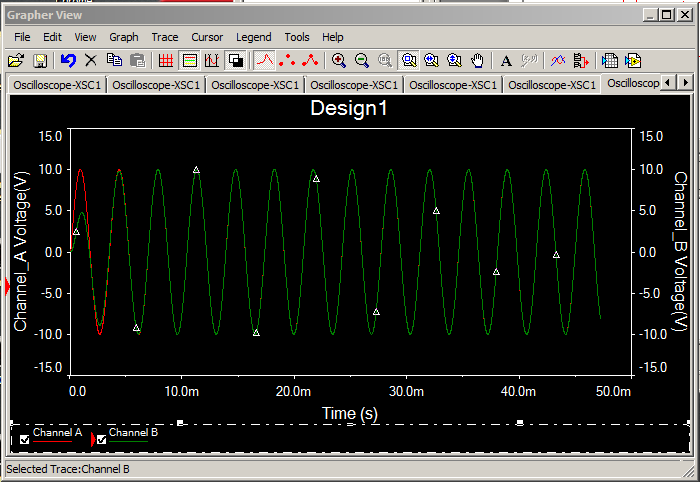
\includegraphics[width=5in]{289hz.PNG} 
   \caption{RLC circuit at 289 Hertz ($w_{n}$)}
   \label{fig:example}
\end{figure}
\bigskip

\begin{figure}[h!] %  figure placement: here, top, bottom, or page
   \centering
   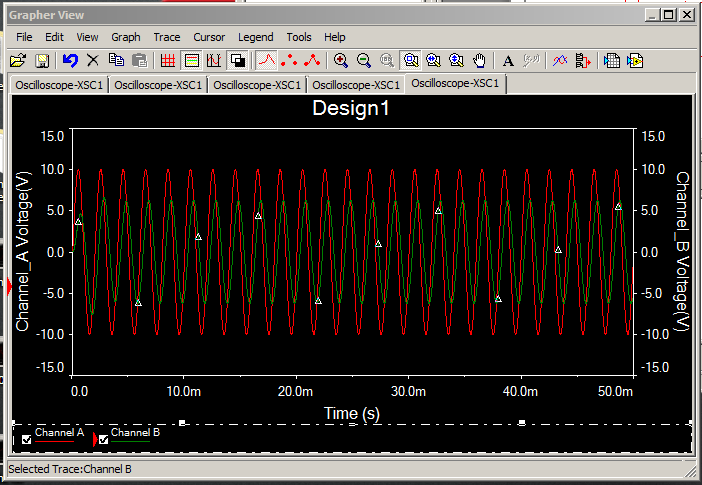
\includegraphics[width=5in]{500hz.PNG} 
   \caption{RLC circuit at 500 Hertz}
   \label{fig:example}
\end{figure}

\newpage

\begin{figure}[h!] %  figure placement: here, top, bottom, or page
   \centering
   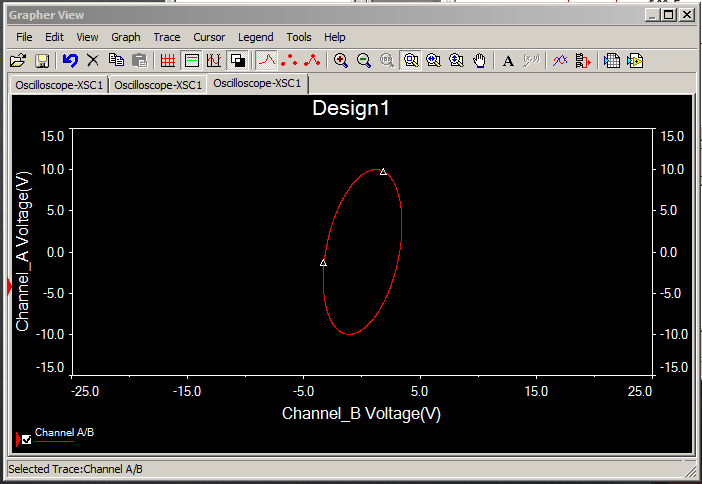
\includegraphics[width=5in]{100hz_ab.PNG} 
   \caption{Input/Output at 100 Hertz}
   \label{fig:example}
\end{figure}
\bigskip

\begin{figure}[h!] %  figure placement: here, top, bottom, or page
   \centering
   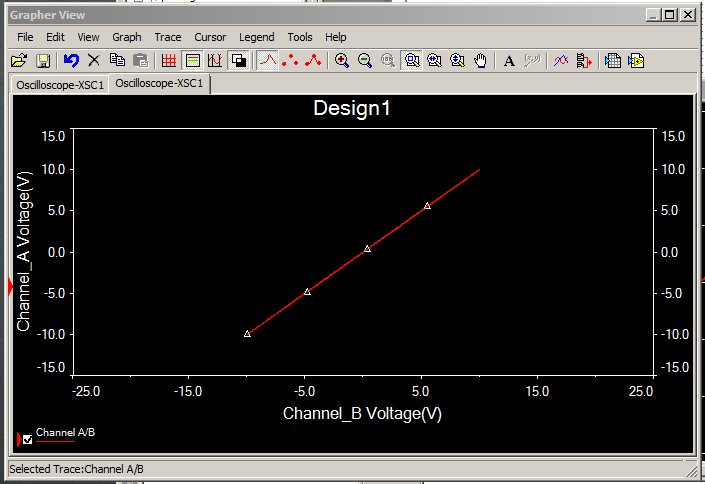
\includegraphics[width=5in]{289hz_ab.PNG} 
   \caption{Input/Output at 289 Hertz ($w_{n}$)}
   \label{fig:example}
\end{figure}

\newpage

\begin{figure}[h!] %  figure placement: here, top, bottom, or page
   \centering
   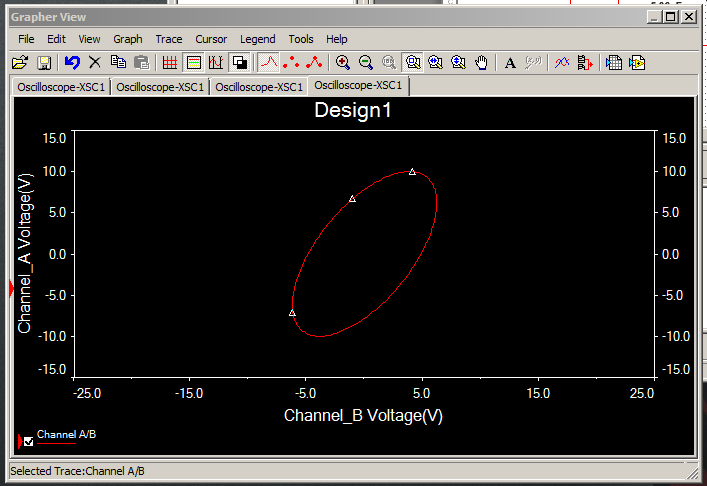
\includegraphics[width=4in]{500hz_ab.PNG} 
   \caption{Input/Output at 500 Hertz}
   \label{fig:example}
\end{figure}
\bigskip

The circuit configuration created in Multisim was then created physically in the lab, as shown in Figure 12. An excel spreadsheet, shown in Figure 13, was used in this lab to aid in calculating values for resistance and capacitance that would match the available inductor for a chosen natural frequency. The values of the individual resistance varied from its denoted value slightly, as is usual with resistors.\bigskip

The input to the circuit was generated with a function generator. The frequency of the input was changed and the output was measured with an oscilloscope, seen in Figures 14 through 16. The input/output graphs were also recorded at different frequencies, shown in Figures17 through 19.

% Lab figures
\begin{figure}[h!] %  figure placement: here, top, bottom, or page
   \centering
   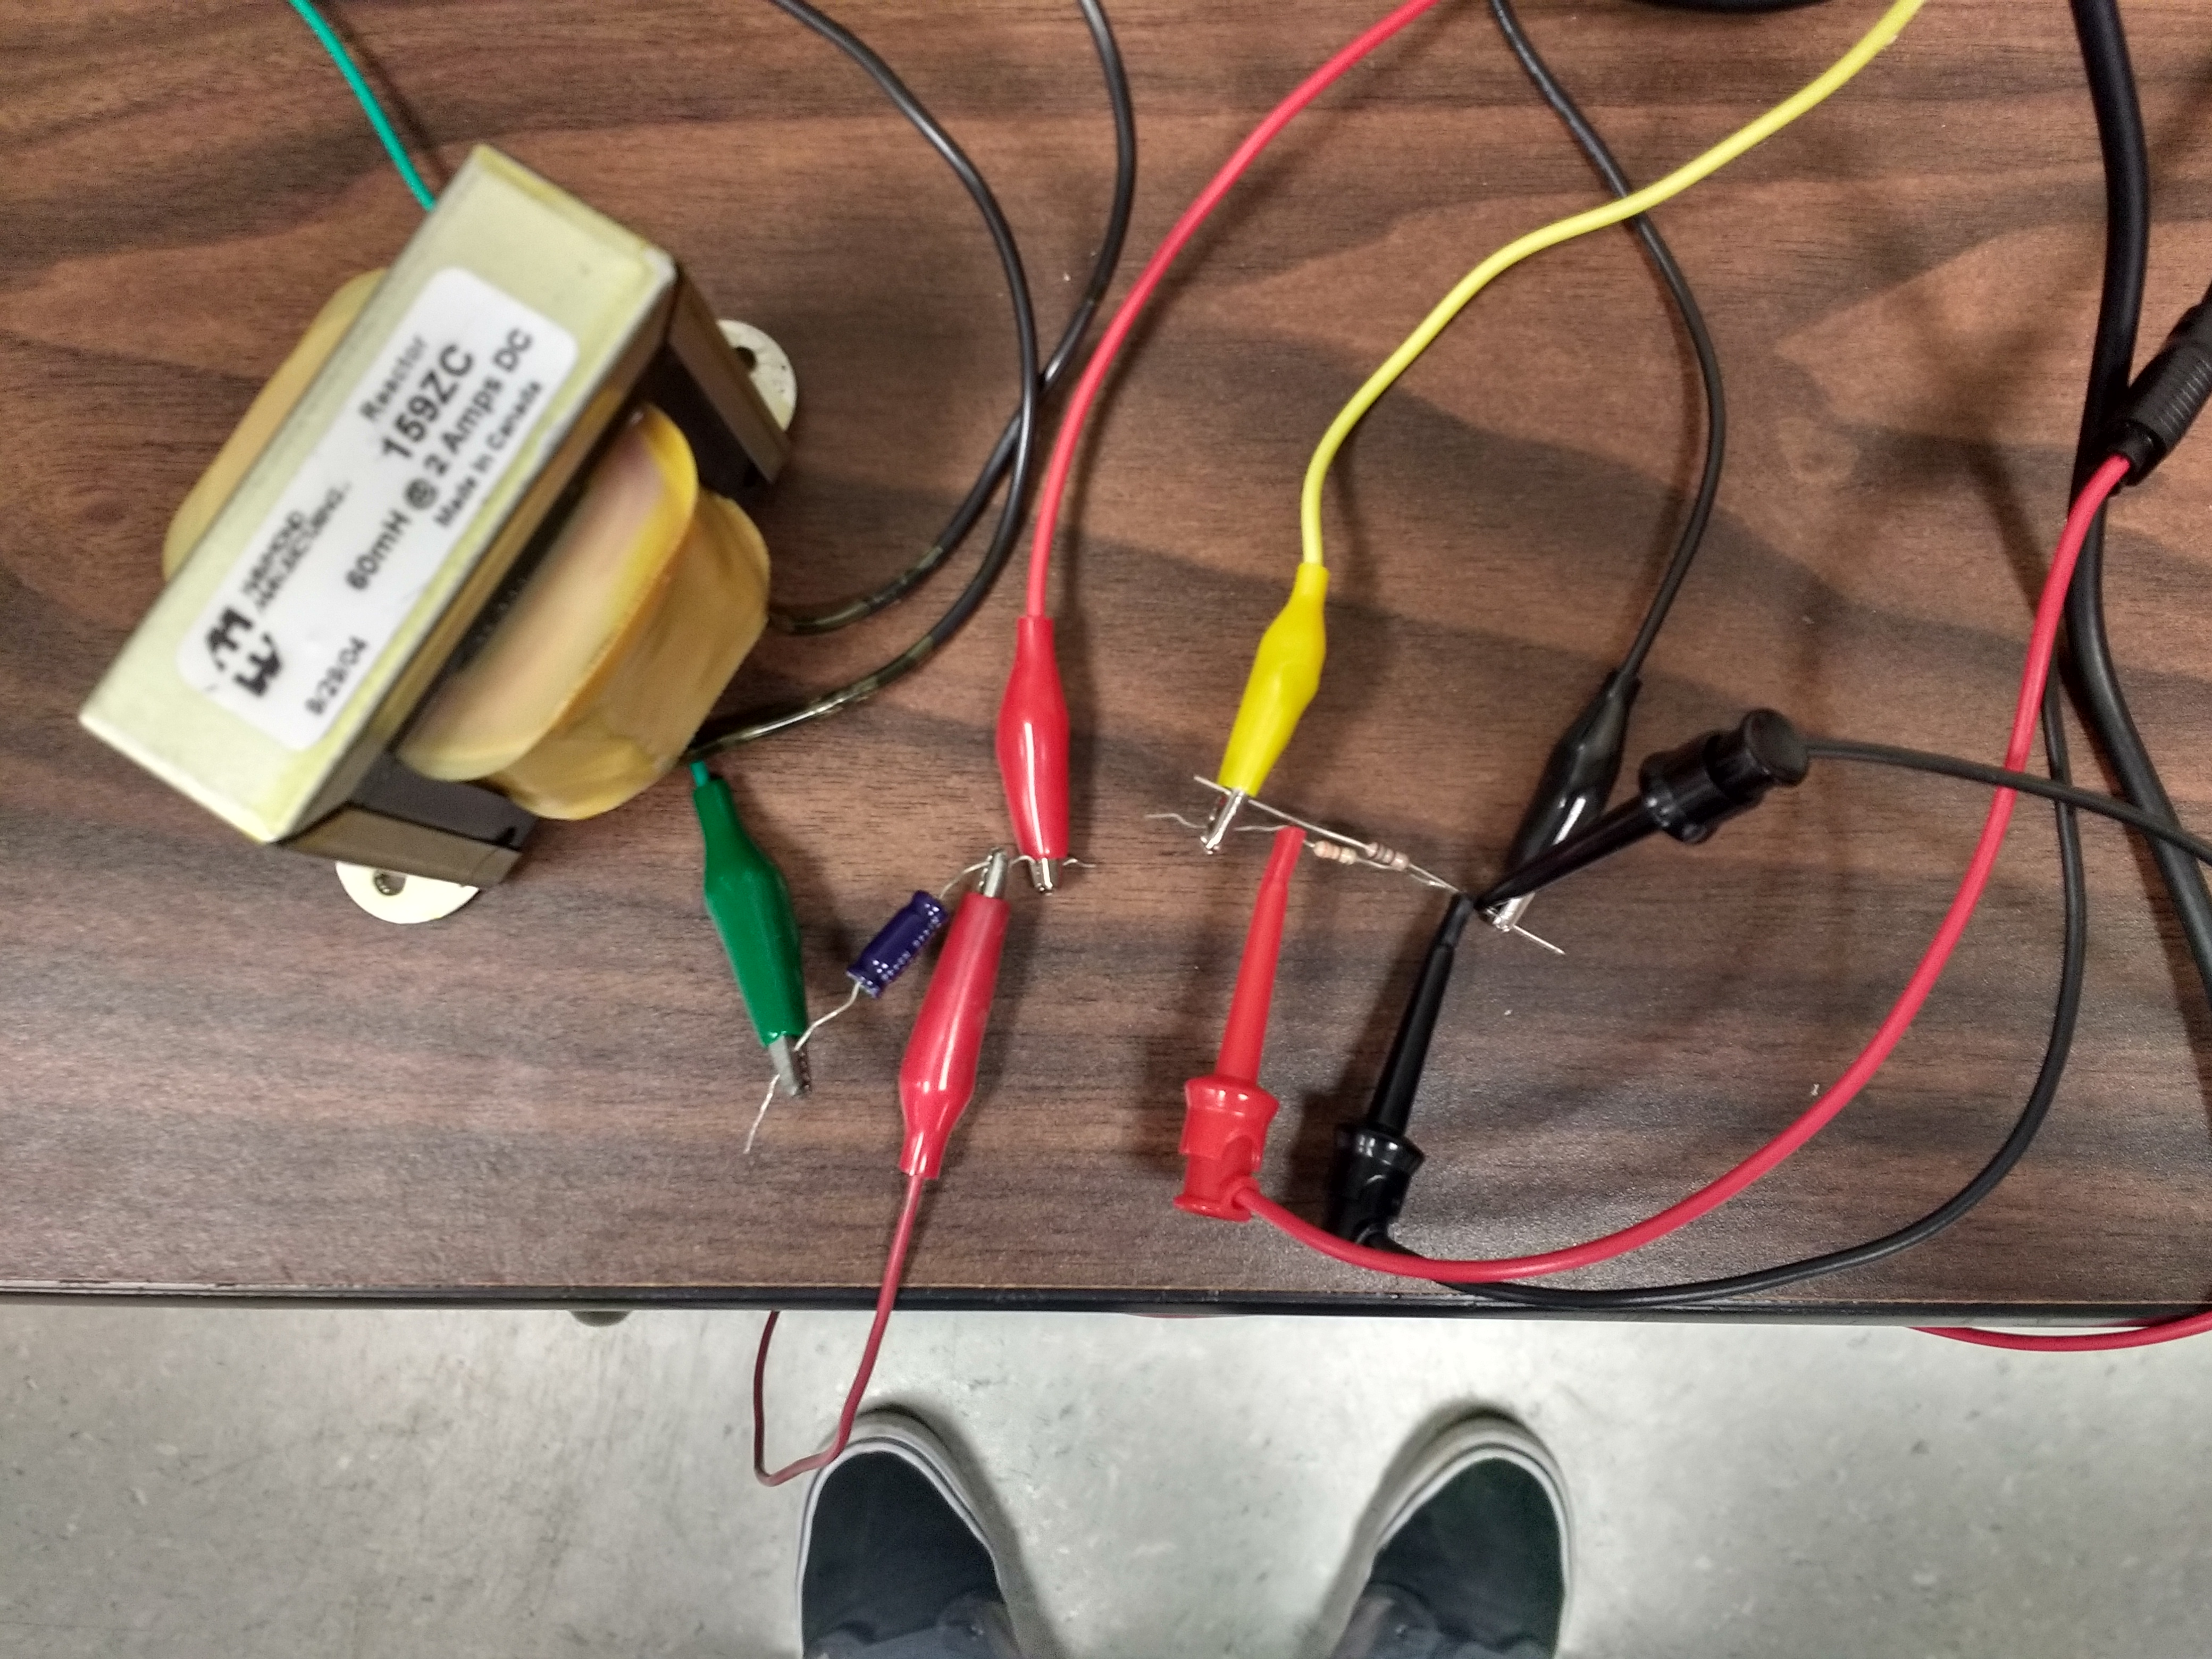
\includegraphics[width=4in]{real_circuit.jpg} 
   \caption{Physical RLC Circuit}
   \label{fig:example}
\end{figure}

\newpage

\begin{figure}[h!] %  figure placement: here, top, bottom, or page
   \centering
   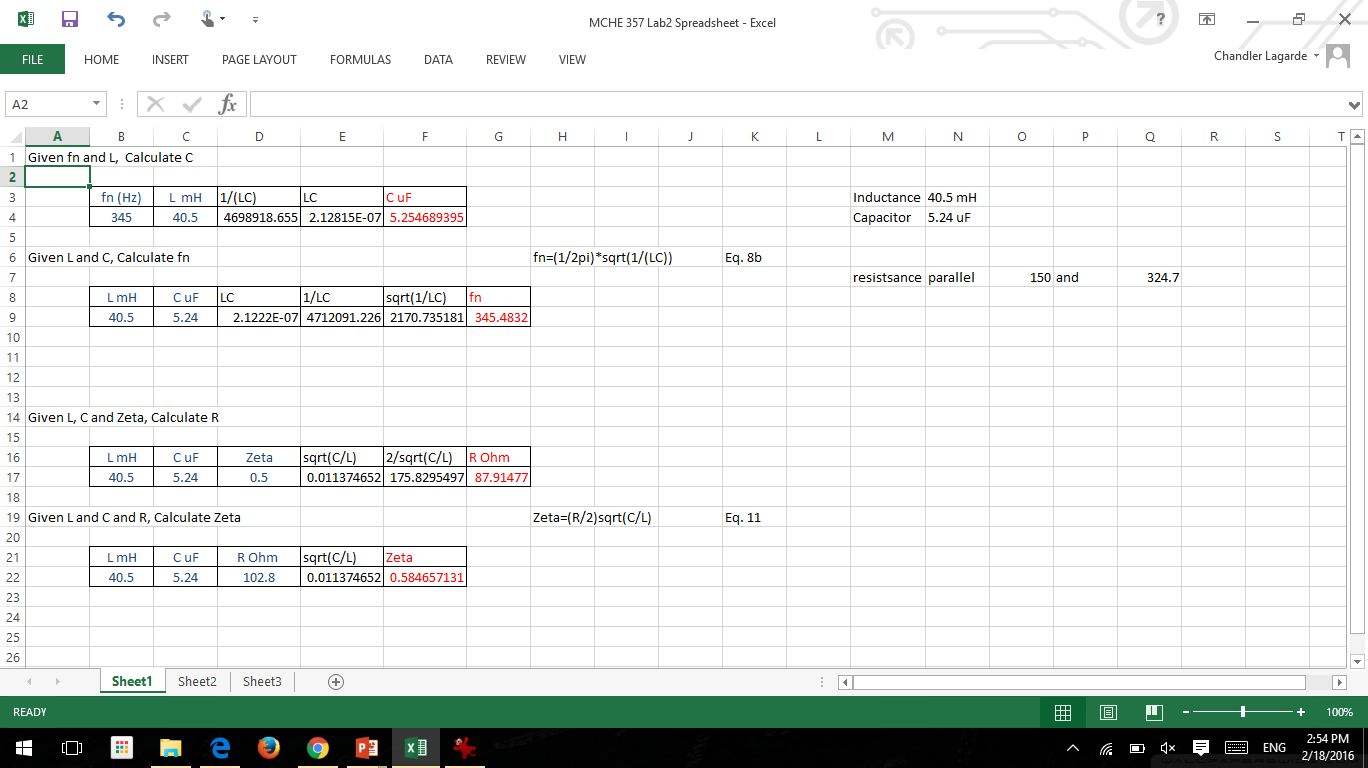
\includegraphics[width=\linewidth]{SpreadSheetFinal.jpg} 
   \caption{Lab Spreadsheet}
   \label{fig:example}
\end{figure}
\bigskip

\begin{figure}[h!] %  figure placement: here, top, bottom, or page
   \centering
   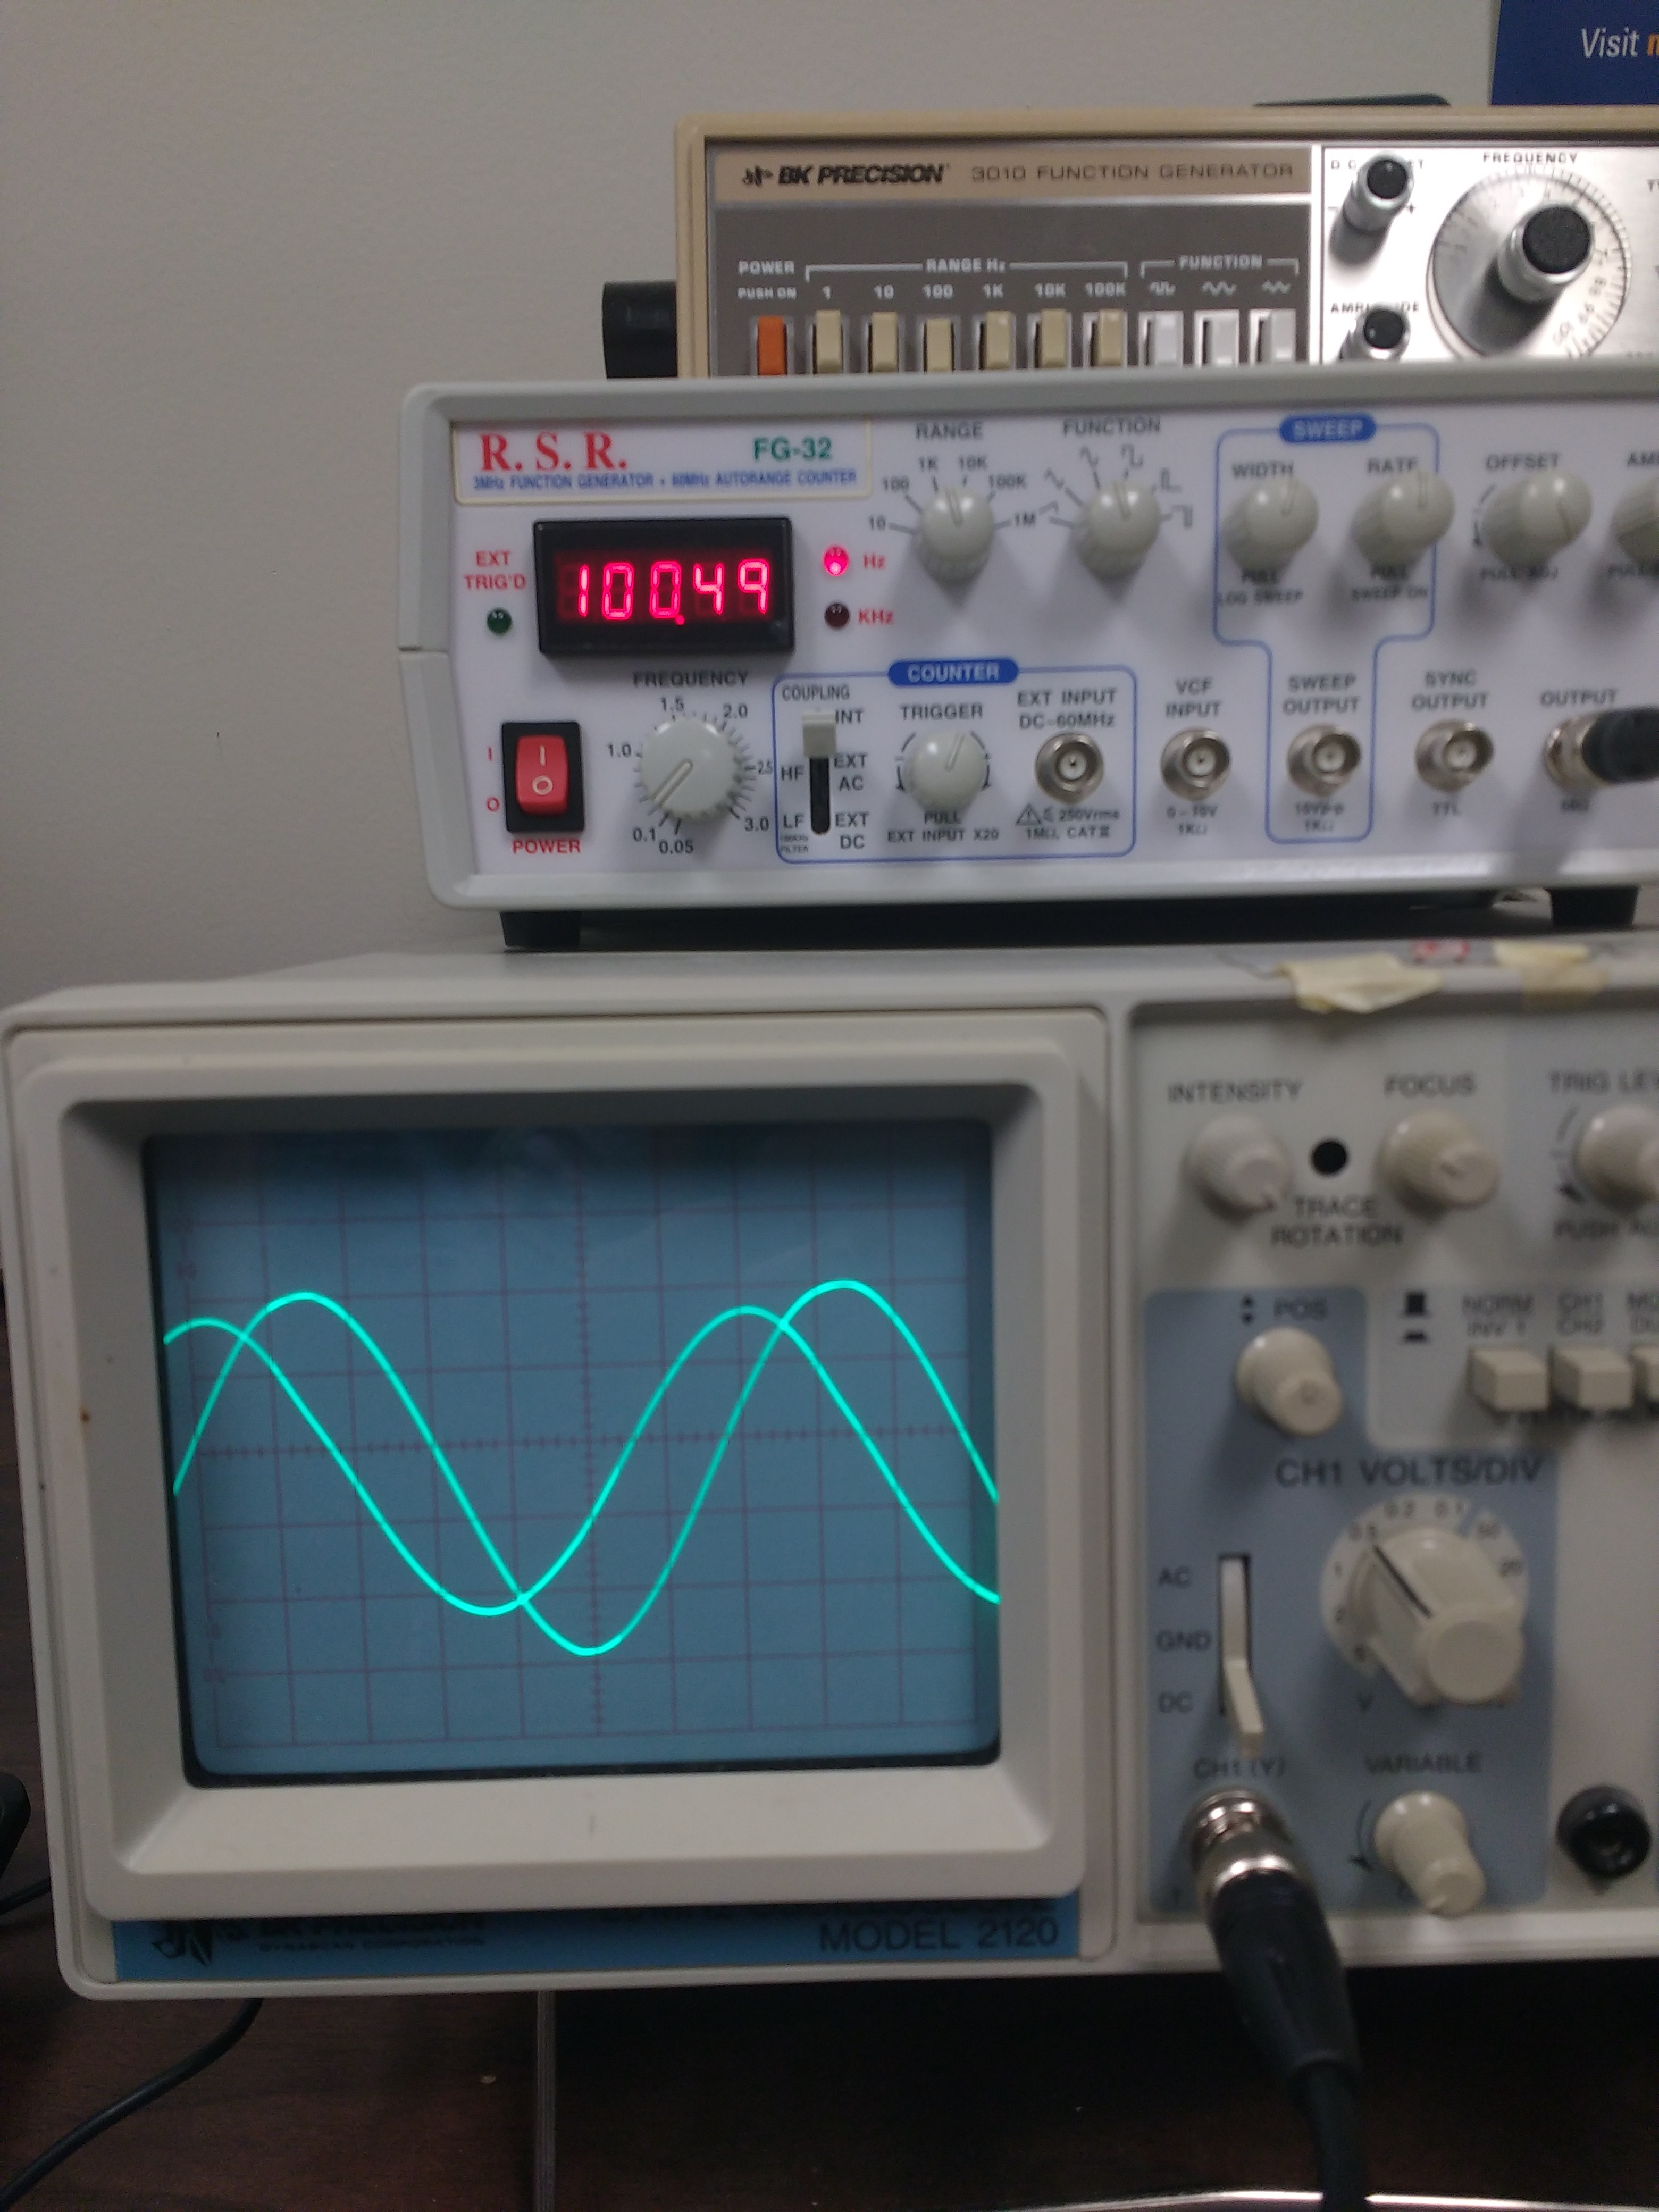
\includegraphics[width=2.5in]{below_nat_freq.jpg} 
   \caption{Oscilloscope reading at 100 Hertz}
   \label{fig:example}
\end{figure}

\newpage

\begin{figure}[h!] %  figure placement: here, top, bottom, or page
   \centering
   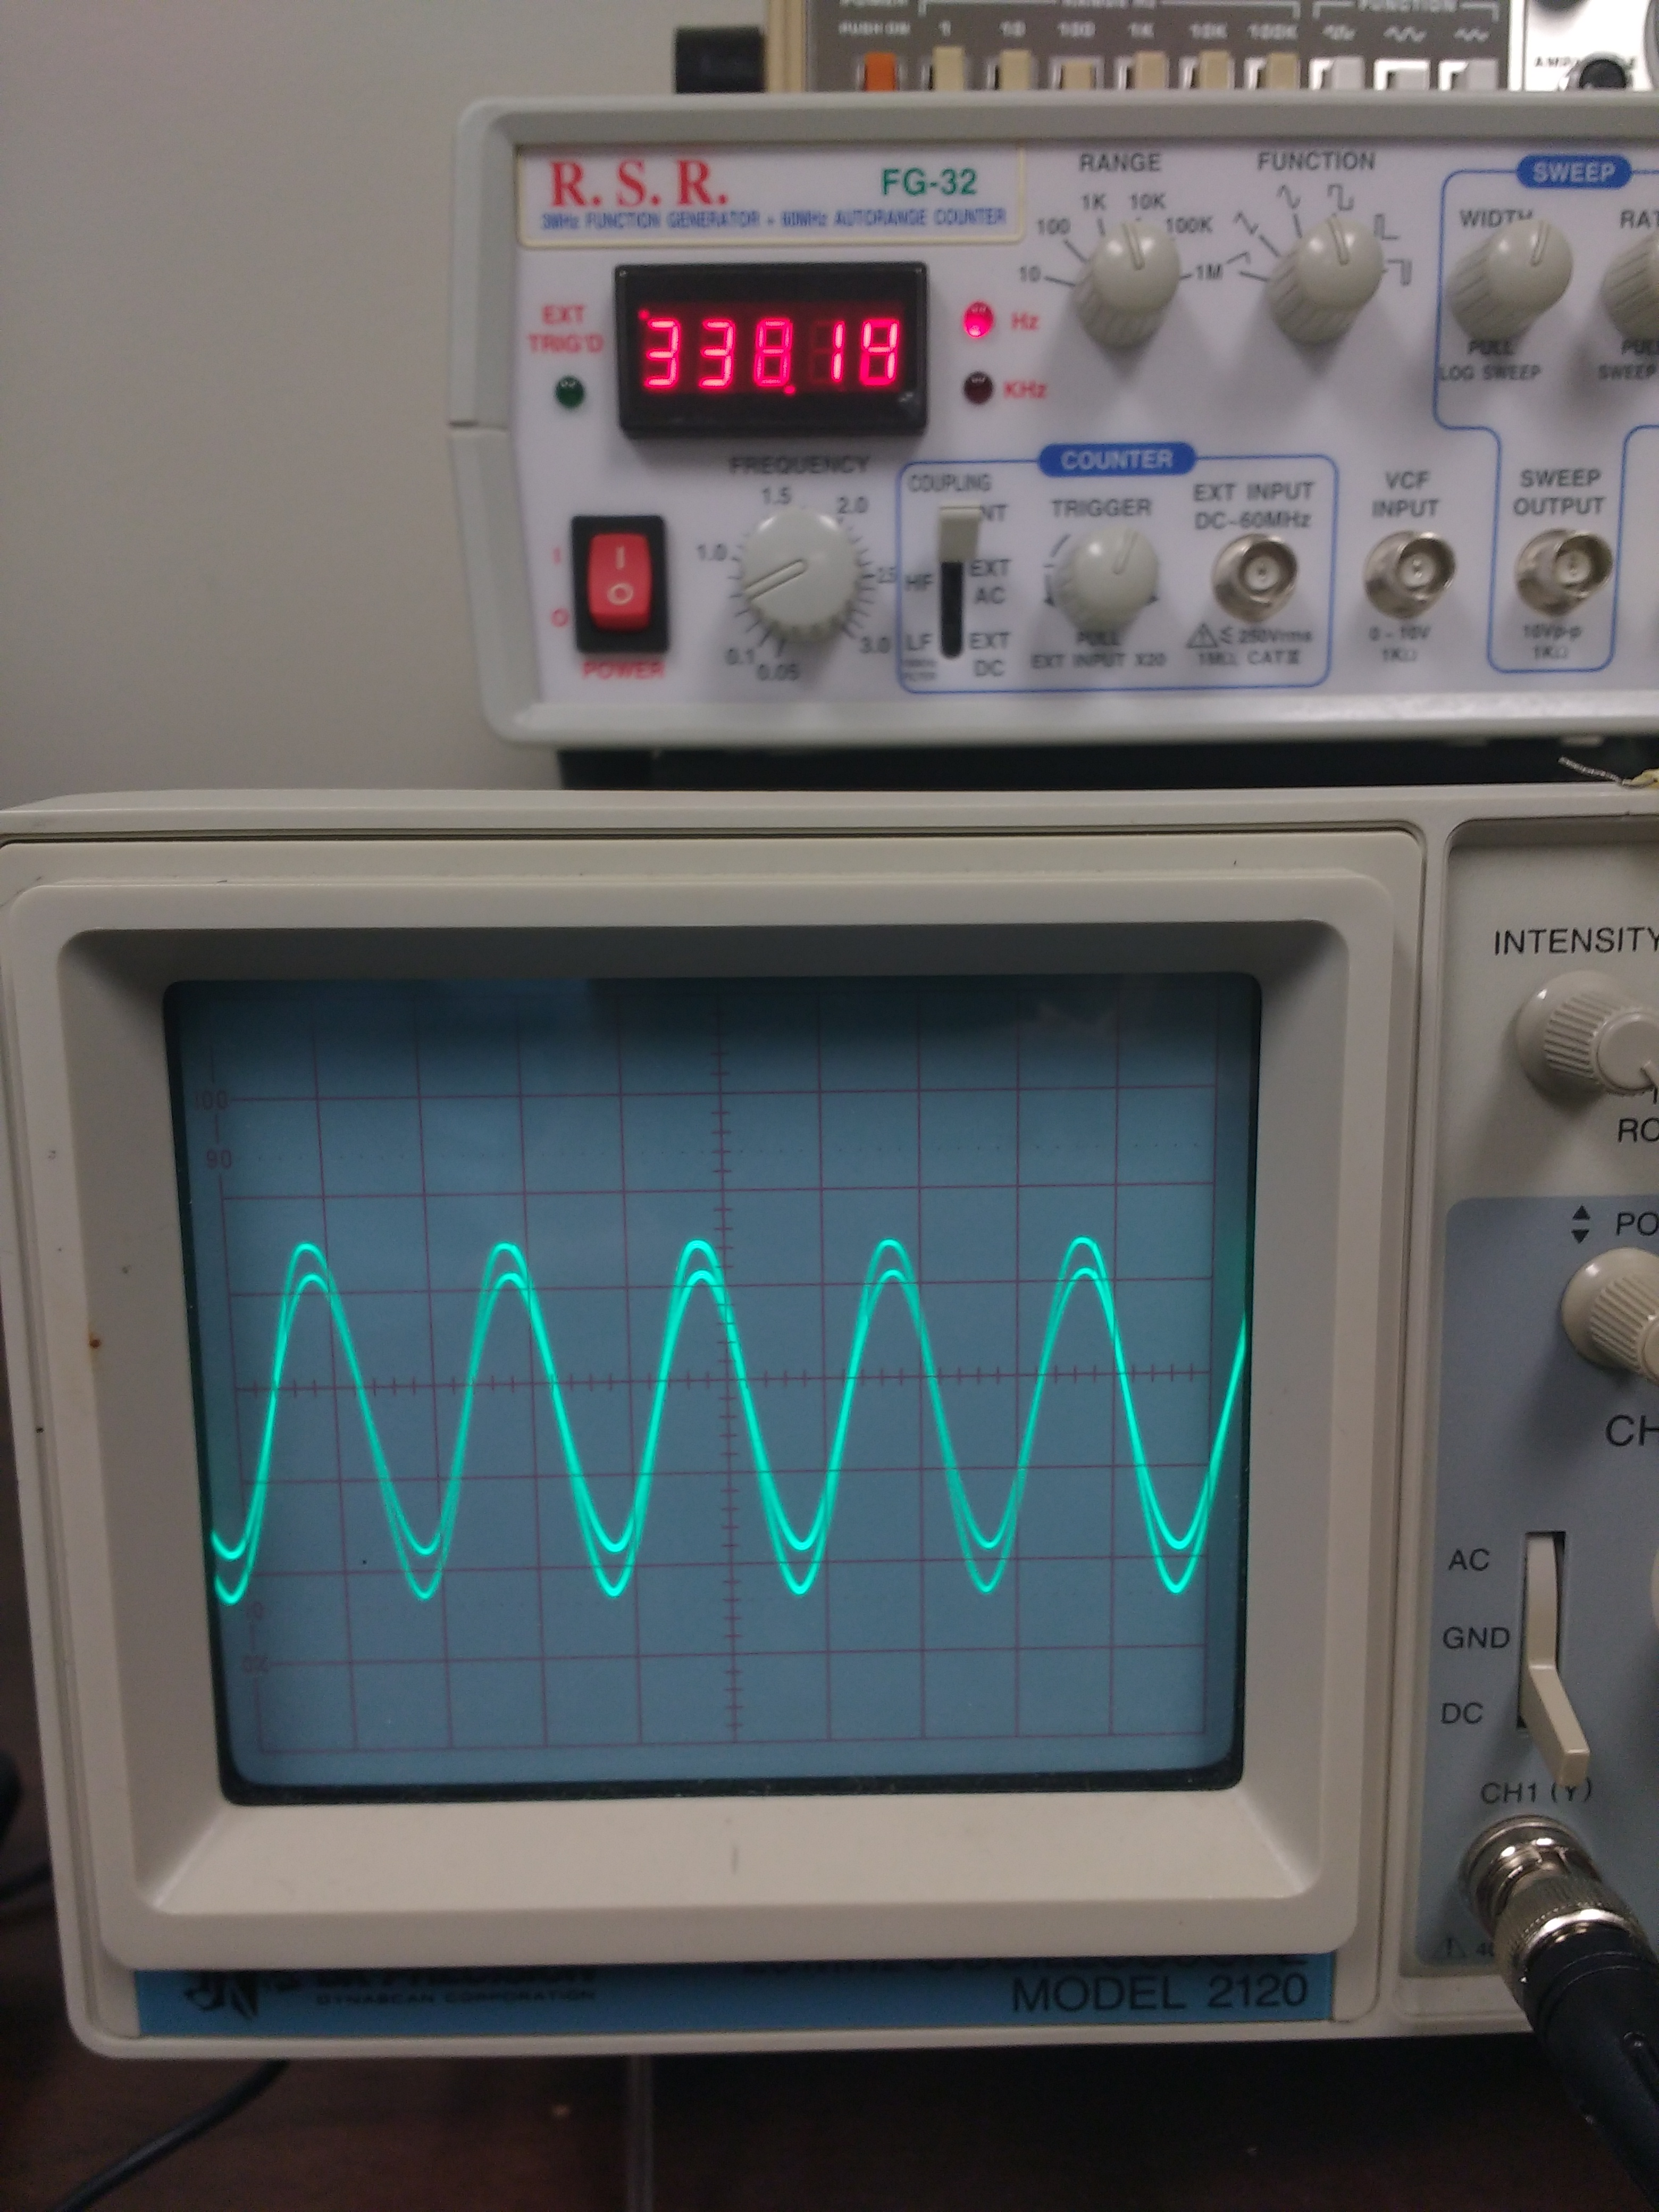
\includegraphics[width=2.5in]{at_nat_freq.jpg} 
   \caption{Oscilloscope reading at 289 Hertz ($w_{n}$)}
   \label{fig:example}
\end{figure}
\bigskip

\begin{figure}[h!] %  figure placement: here, top, bottom, or page
   \centering
   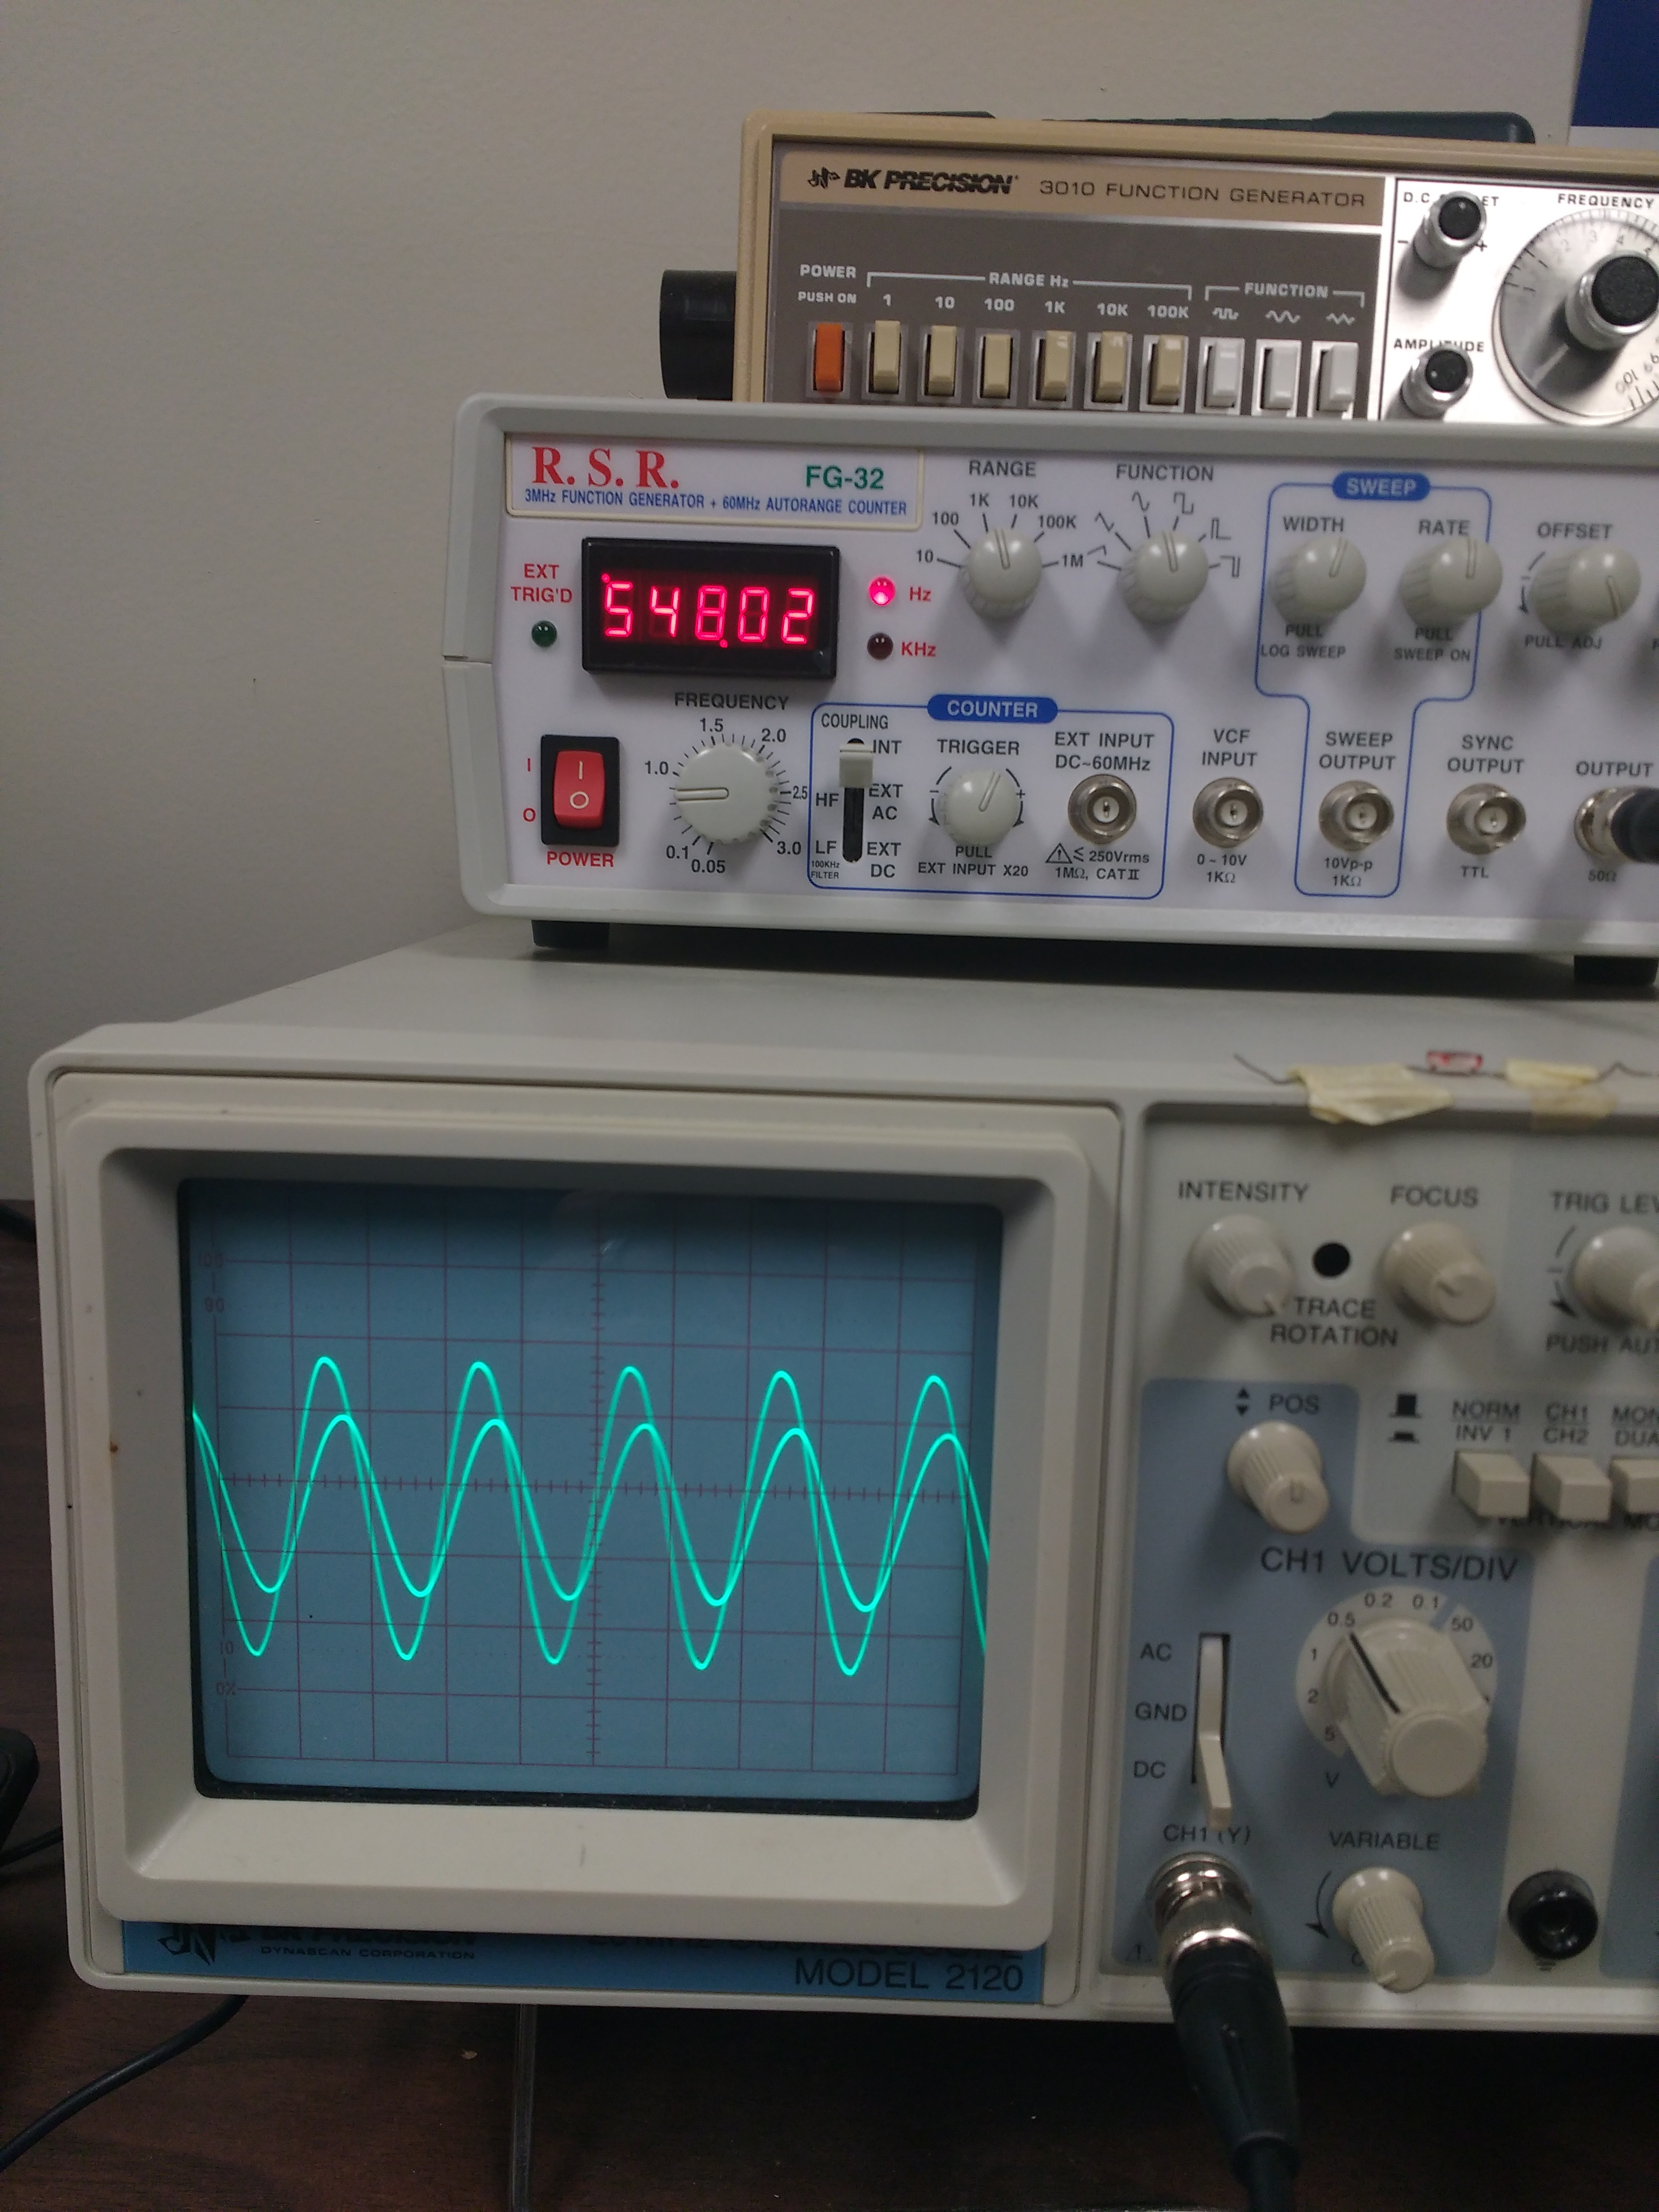
\includegraphics[width=2.5in]{above_nat_freq.jpg} 
   \caption{Oscilloscope reading at 500 Hertz}
   \label{fig:example}
\end{figure}

\newpage

\begin{figure}[h!] %  figure placement: here, top, bottom, or page
   \centering
   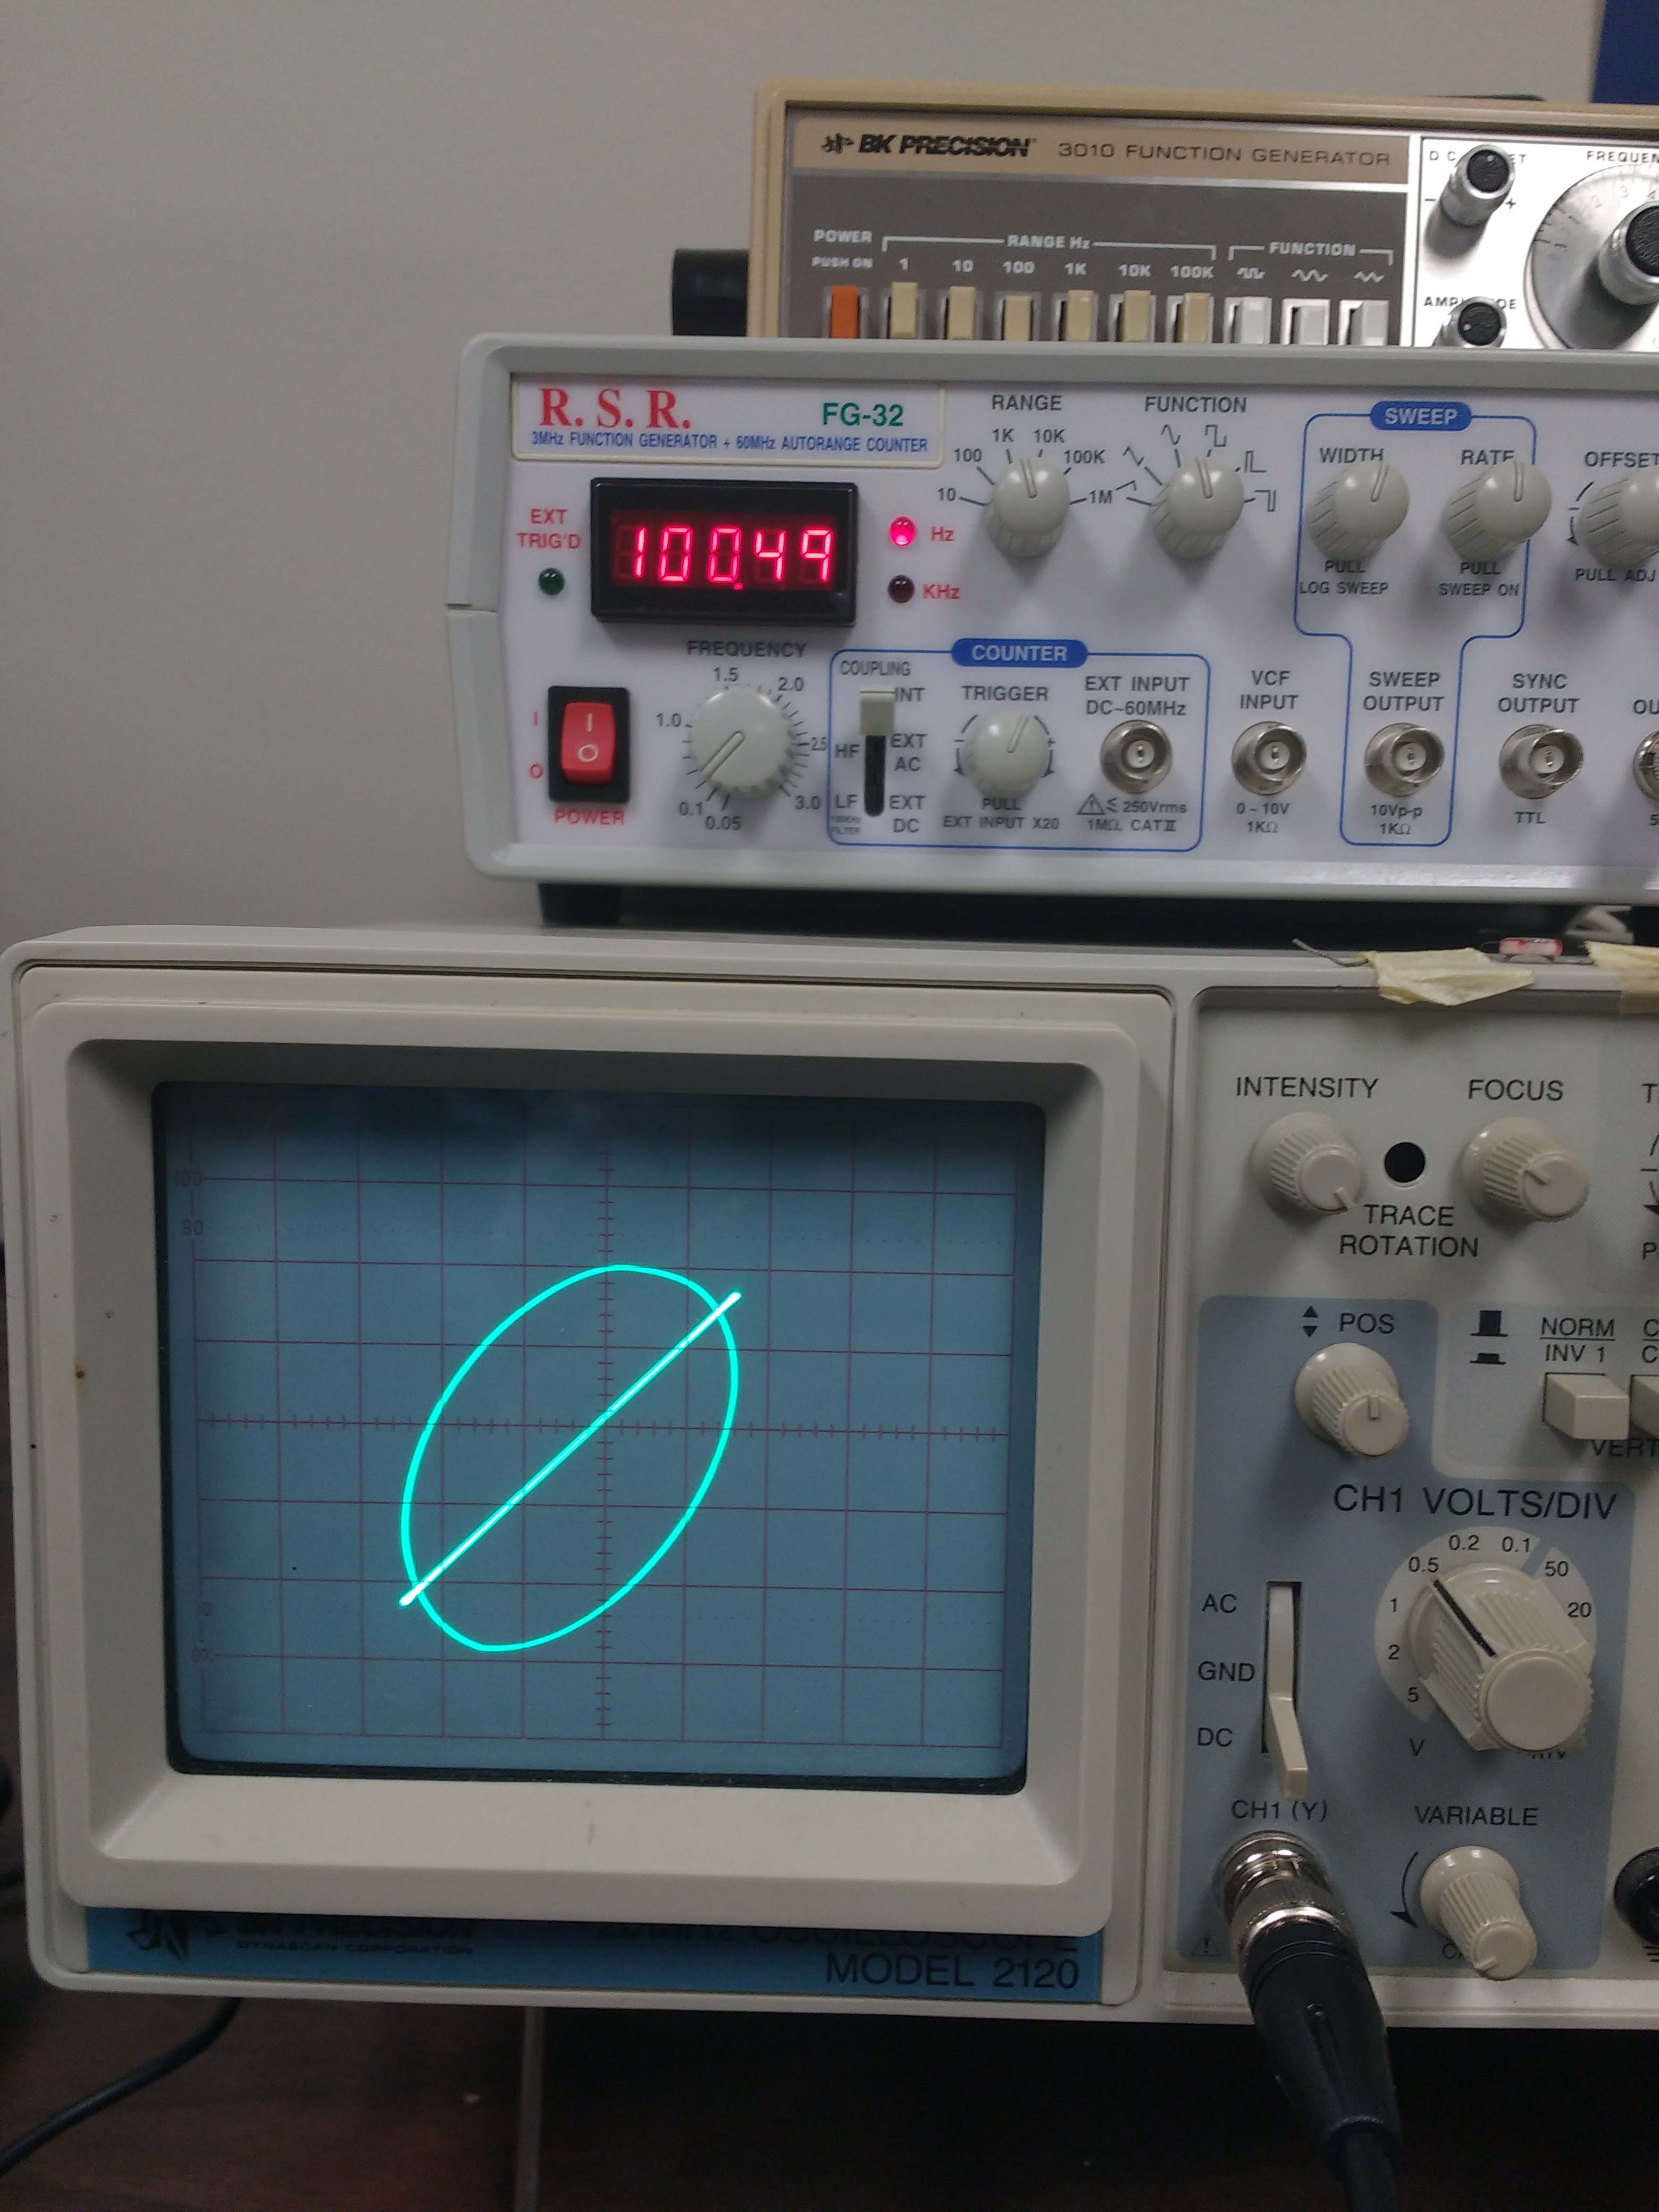
\includegraphics[width=2.5in]{ab_below_nat_freq.jpg} 
   \caption{Oscilloscope Input/Output reading at 100 Hertz}
   \label{fig:example}
\end{figure}
\bigskip

\begin{figure}[h!] %  figure placement: here, top, bottom, or page
   \centering
   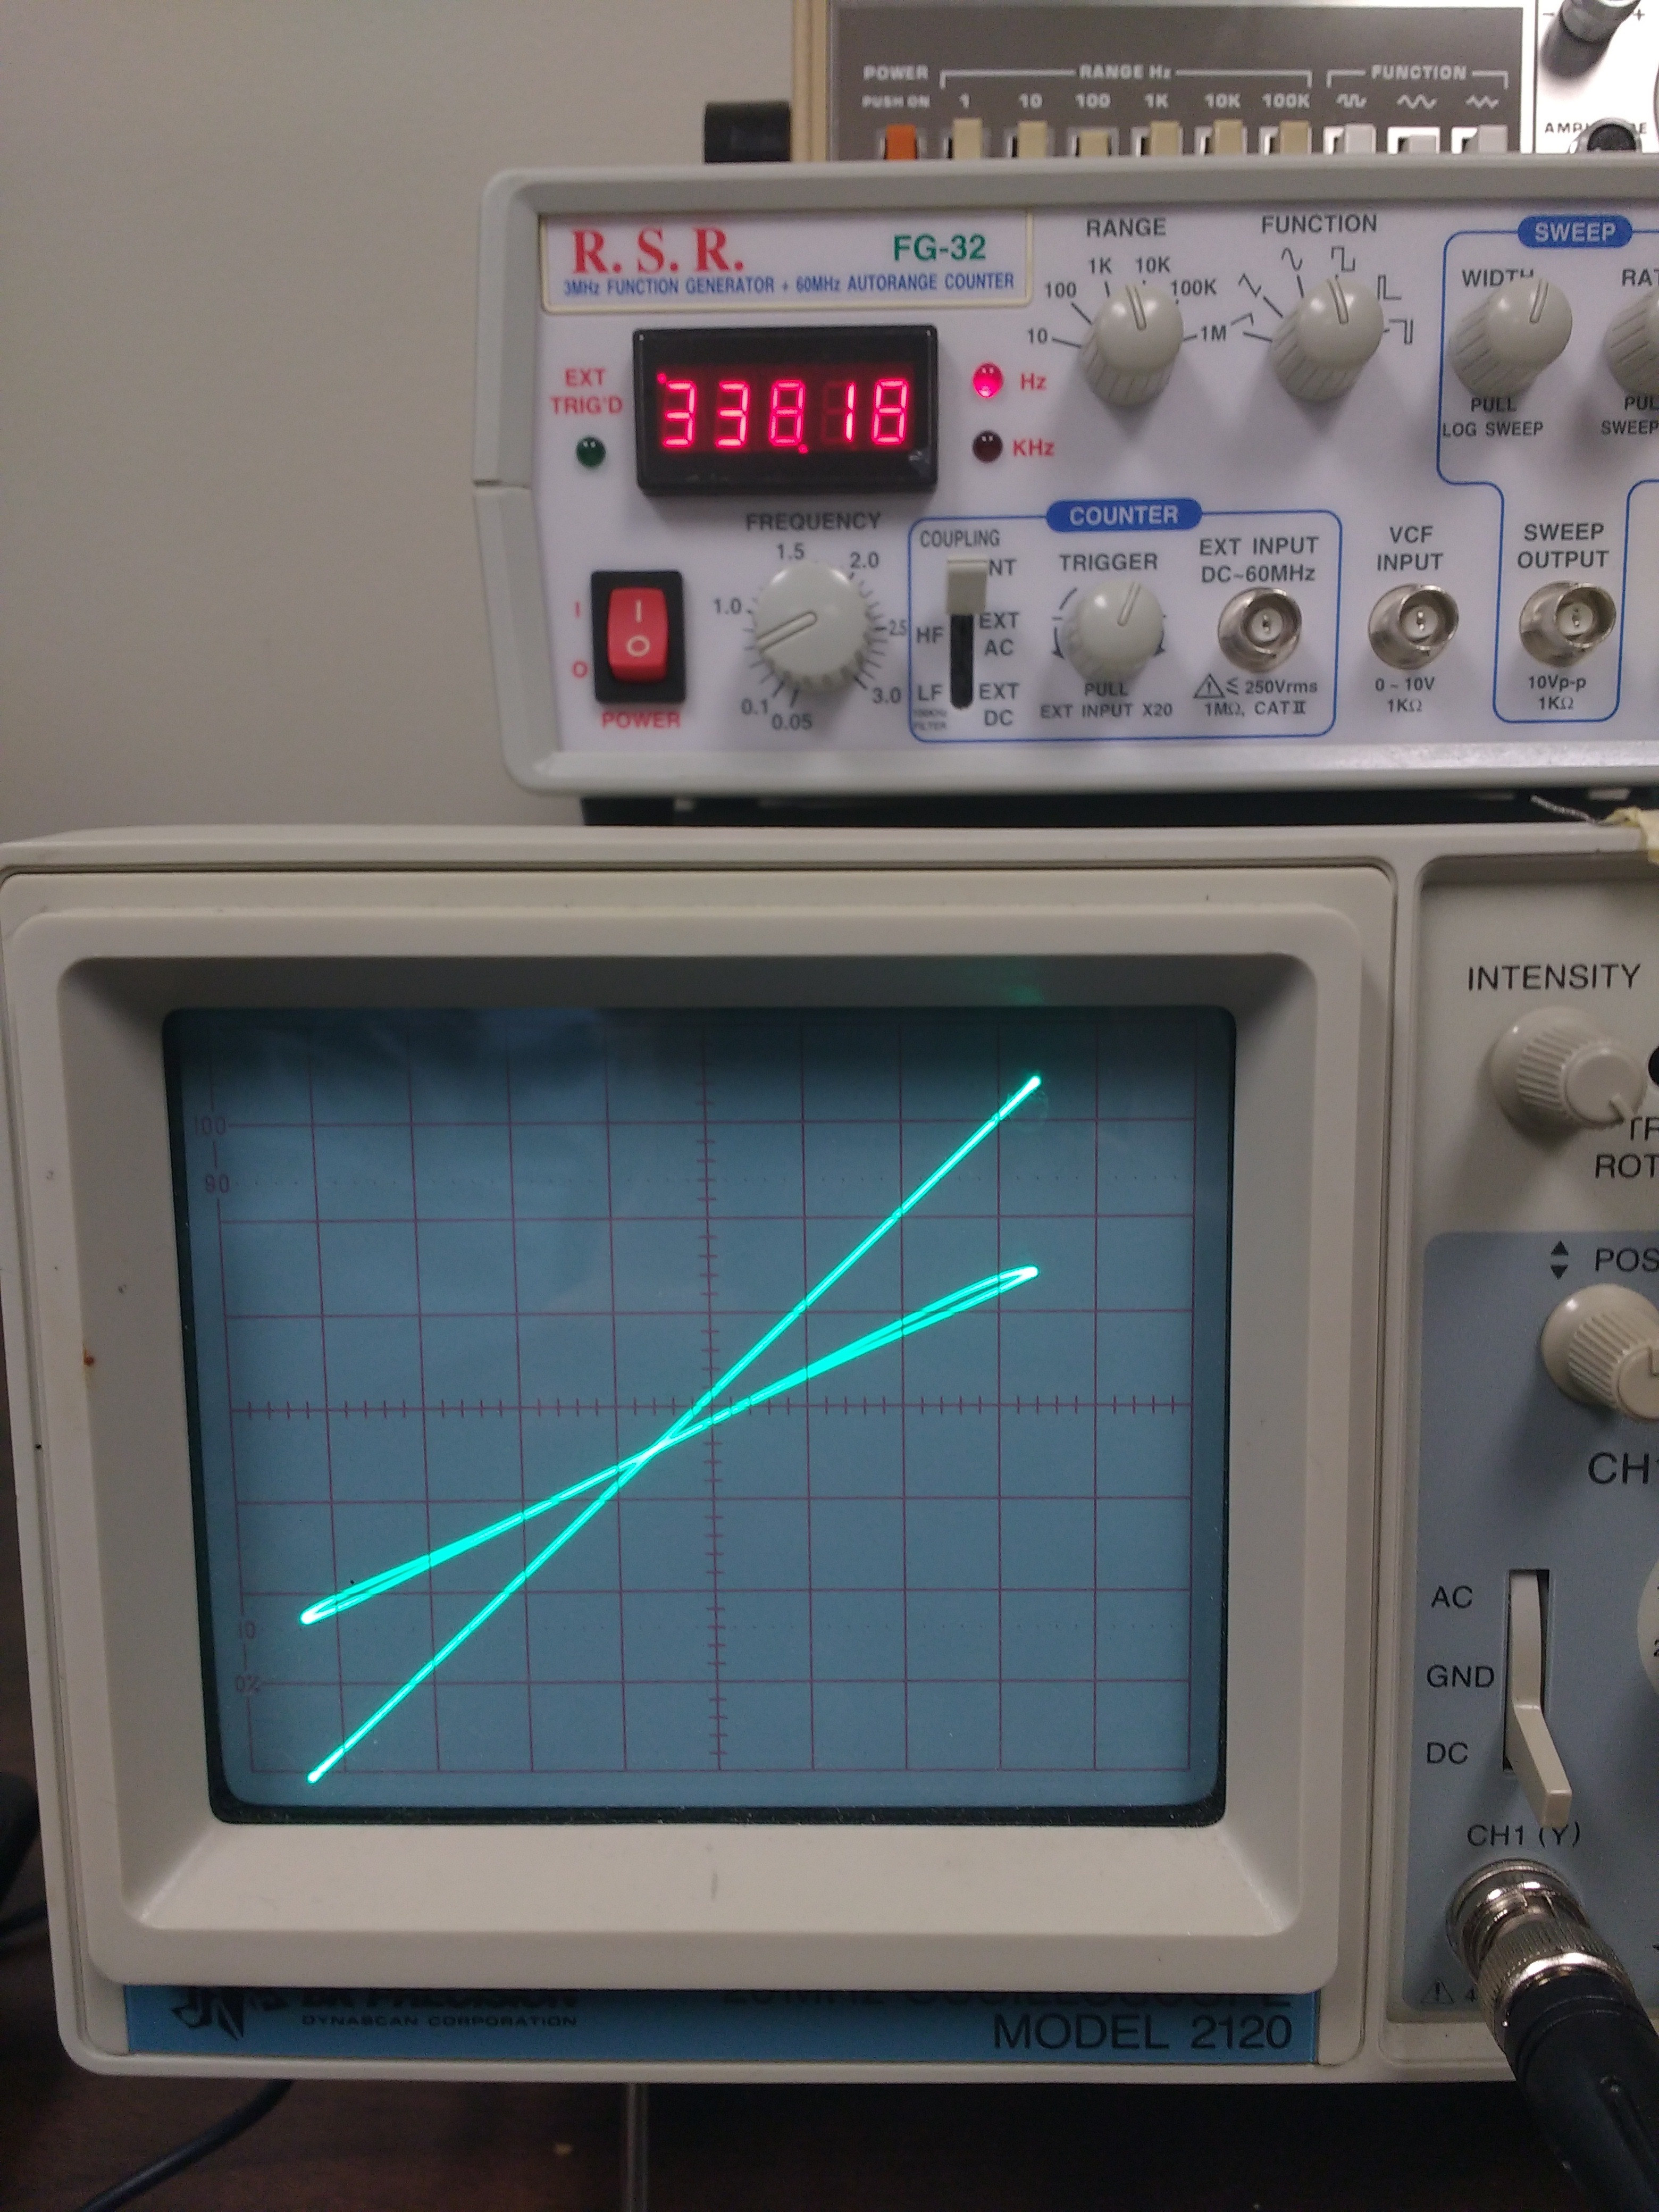
\includegraphics[width=2.5in]{ab_at_nat_freq.jpg} 
   \caption{Oscilloscope Input/Output reading at 289 Hertz ($w_{n}$)}
   \label{fig:example}
\end{figure}

\newpage

\begin{figure}[h] %  figure placement: here, top, bottom, or page
   \centering
   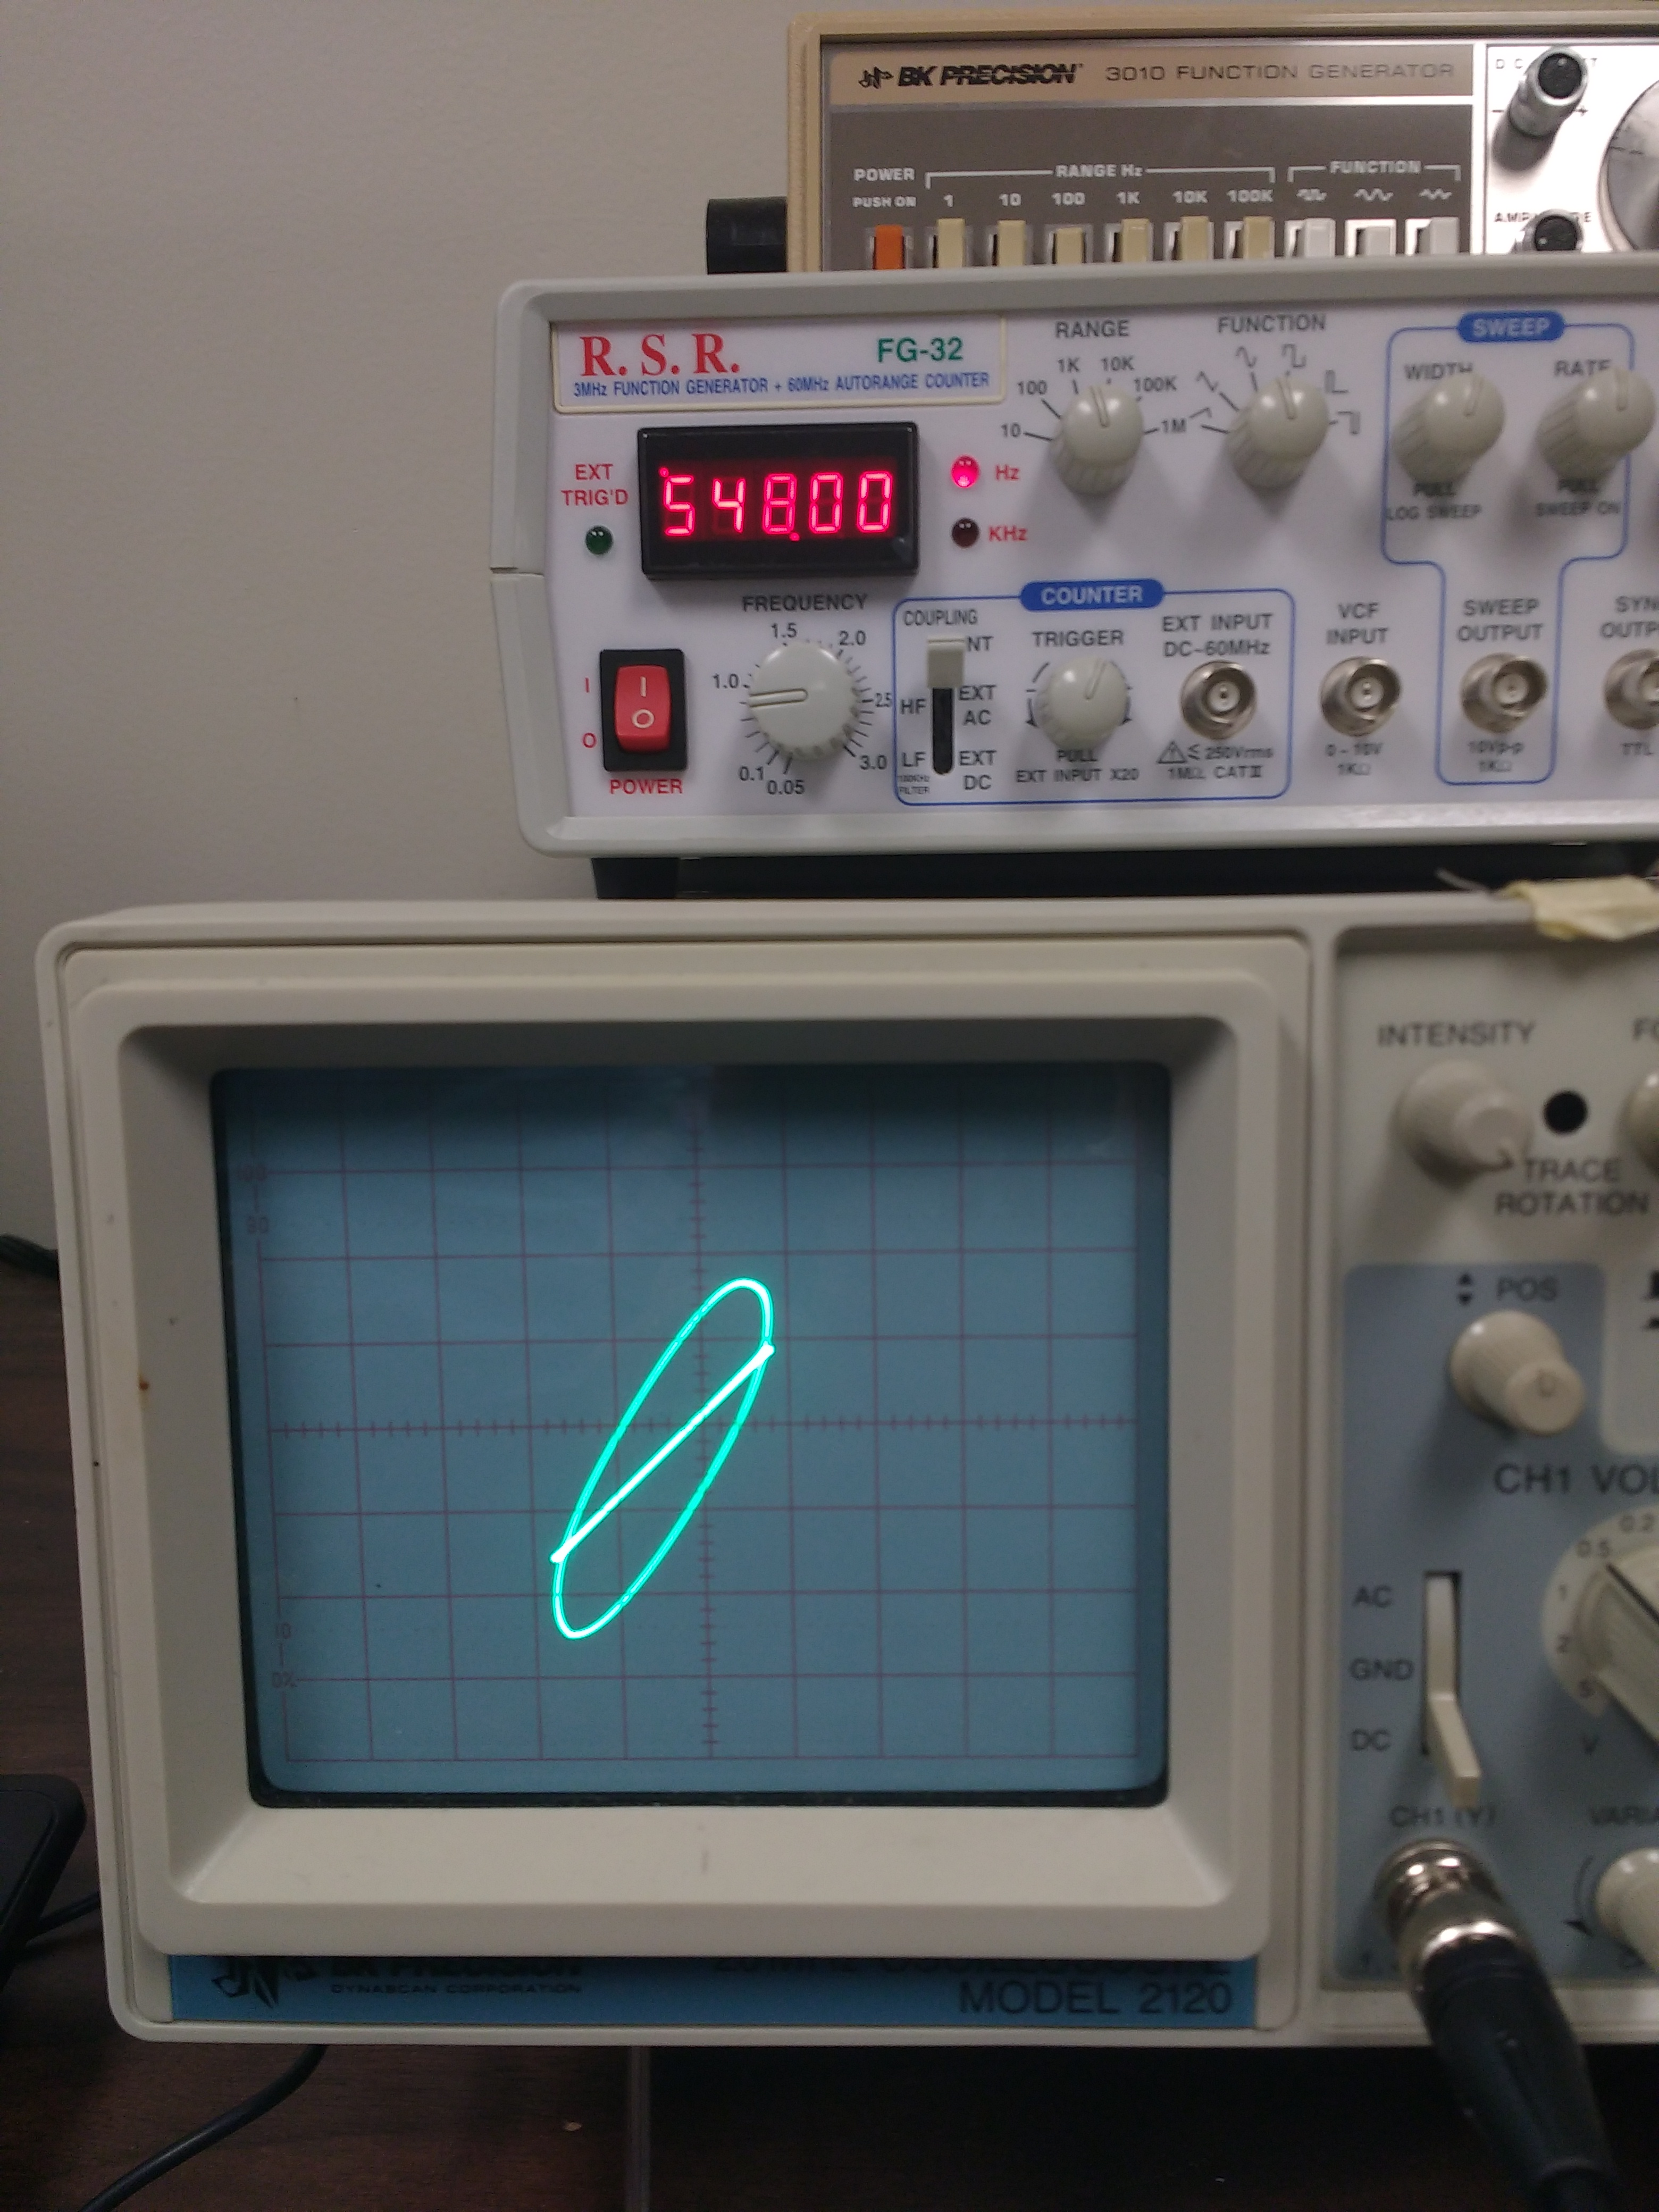
\includegraphics[width=2.5in]{ab_above_nat_freq.jpg} 
   \caption{Oscilloscope Input/Output reading at 500 Hertz}
   \label{fig:example}
\end{figure}
\bigskip



\section*{\fontsize{12}{12}\selectfont \large Conclusion}
\addcontentsline{toc}{section}{Conclusion} % Add for each section
This lab demonstrated the principles of basic RLC circuits. These devices include resistances, capacitors, and inductances. The effects of varying the resistance and input frequency were studied. It was noted that these circuits behave very analogously to the basic vibration system consisting of a mass, spring, and damper. It was also seen how these circuits can be used in many devices commonly used in everyday life.



%\section*{\fontsize{12}{12}\selectfont \large References}

\begin{thebibliography}{2}

% Example
%\bibitem{Wagner}
%Ng, K., Wagner, S.W., Camelio, J., Emblom, W.J. (2010). ?Experimental Analysis of Micro Tube
%Hydroforming Process.? Transactions of NAMRC of SME, 38, 577-584.

\end{thebibliography}



%\section*{\fontsize{12}{12}\selectfont APPENDIX}

%\begin{table}[h!]
%  \caption{}
%  \includegraphics[width=\linewidth]{table1.png}
%\end{table}




\end{document}







----------------------------Templates-------------------------------

-------------------------Figure-----------------------

\begin{figure}[h!]  
  \centering
    \includegraphics[width=\linewidth]{**file**}
    \caption{Docking Station}
\end{figure}

---------------------------Table-----------------------
\begin{table}[ht]
\caption{Nonlinear Model Results} % title of Table
\centering % used for centering table
\begin{tabular}{c c c c} % centered columns (4 columns)
\hline\hline %inserts double horizontal lines
Case & Method\#1 & Method\#2 & Method\#3 \\ [0.5ex] % inserts table
%heading
\hline % inserts single horizontal line
1 & 50 & 837 & 970 \\ % inserting body of the table
2 & 47 & 877 & 230 \\
3 & 31 & 25 & 415 \\
4 & 35 & 144 & 2356 \\
5 & 45 & 300 & 556 \\ [1ex] % [1ex] adds vertical space
\hline %inserts single line
\end{tabular}
\label{table:nonlin} % is used to refer this table in the text
\end{table}



probably best to insert as an image from excel

\bigskip\\
\begin{table}[h!]
  \caption{}
  \includegraphics[width=\linewidth]{**file**}
\end{table}
\bigskip\\





-----------------------------Equations------------------------
-----------------------------Regular
\begin{equation}
a = b + c
\end{equation}

--------------------------------- Multiline
\begin{multline}
a = b + c + d + e + f
+ g + h + i + j \\
+ k + l + m + n + o
\end{multline}

-------------------------------Citations-------------------------
\bibitem{Author last name}
  Last, First., year of publication,
  article name, book(etc) name, from \\
  link goes here

----------------------------------other-----------------------------

equations:
http://moser-isi.ethz.ch/docs/typeset_equations.pdf

citations:
http://library.missouri.edu/engineering/about/guides/asme
https://www.asme.org/shop/proceedings/conference-publications/references